\chapter{Results and Discussion}
\label{cha:results}

The problem at hand along with the methodology employed to produce the solution are now well defined. Paired with an understanding of important previous works in this area and the technologies available, the design of each of the components may be given consideration. This chapter will present the designs of the required additions to the Gene-Plex Extractor, as were defined in Section \ref{sec:intro_scope}, Scope. This will include relevant results from stages of the design process, the conducted simulations along with validations and verifications via experimental methods. Through the sections below, the reader will be familiar with the design of each of the components along with the resulting performance of the realised and implemented component.\\

\section{Processor Module}

\subsection{Hardware}

\subsubsection{Thermal Isolation}
\label{sec:isolation}

The first consideration given to the design of the physical Processor Module was the thermal isolation of the heated and non-heated volumes. While there is no requirement stipulating that only tubes 2 and 3 may be heated, it was deemed  thermally inefficient to heat the entire module. Such a design would also decrease the performance of the controller due to the larger mass to be heated. Therefore, the module was split into two regions, refereed to as the Thermal Region and the Carrier. While the method of isolation needed to be effective to create a stable and controllable thermal system, a number of other design considerations were present:
\begin{enumerate}
	\item[Manufacturability] The design of the thermal isolation method needed to consider the available manufacturing methods and their capabilities. For example, concept A shown in Figure \ref{fig:splitconcepts}, utilized a simple "trench" to create an air gap between the heated and non-heated regions of a single block of aluminium. While this concept satisfied the serviceability and cost objectives, there were a number of physical constraints preventing it from being feasible. Due to the geometry of the cassettes, the trench width was limited to 3mm across. At this size, the maximum depth at which the tooling could cut was stated to be 30mm \cite{Sorenson}. At this depth, not only would a large area of material still connect the two regions, but the cost of machining would be high.
	\item[Serviceability] When considering the serviceability of the product, two main aspects were key. This includes the initial assembly of the device after manufacture along with the periodic maintenance during its operating life. The resulting design must ensure manual assembly is practical and that the replacement of components, such as sensors or heating hardware is considered. 
	\item[Cost] Given that a total of 3 Processor Modules are required for each Gene-Plex Extractor, the designs selected must be cost effective. while a number of high cost manufacturing methods or materials may have met the needs of the thermal isolation requirement, the cumulative cost required led to a need for alternative concepts to be generated.
\end{enumerate}	

With these factors in mind, four main concepts were generated with the goal of insulating the thermally controlled region of the Processor Module from the non-heated portion in mind. These concepts are displayed in Figure \ref{fig:splitconcepts}.\\

\begin{figure}[!htb]
	\centering
	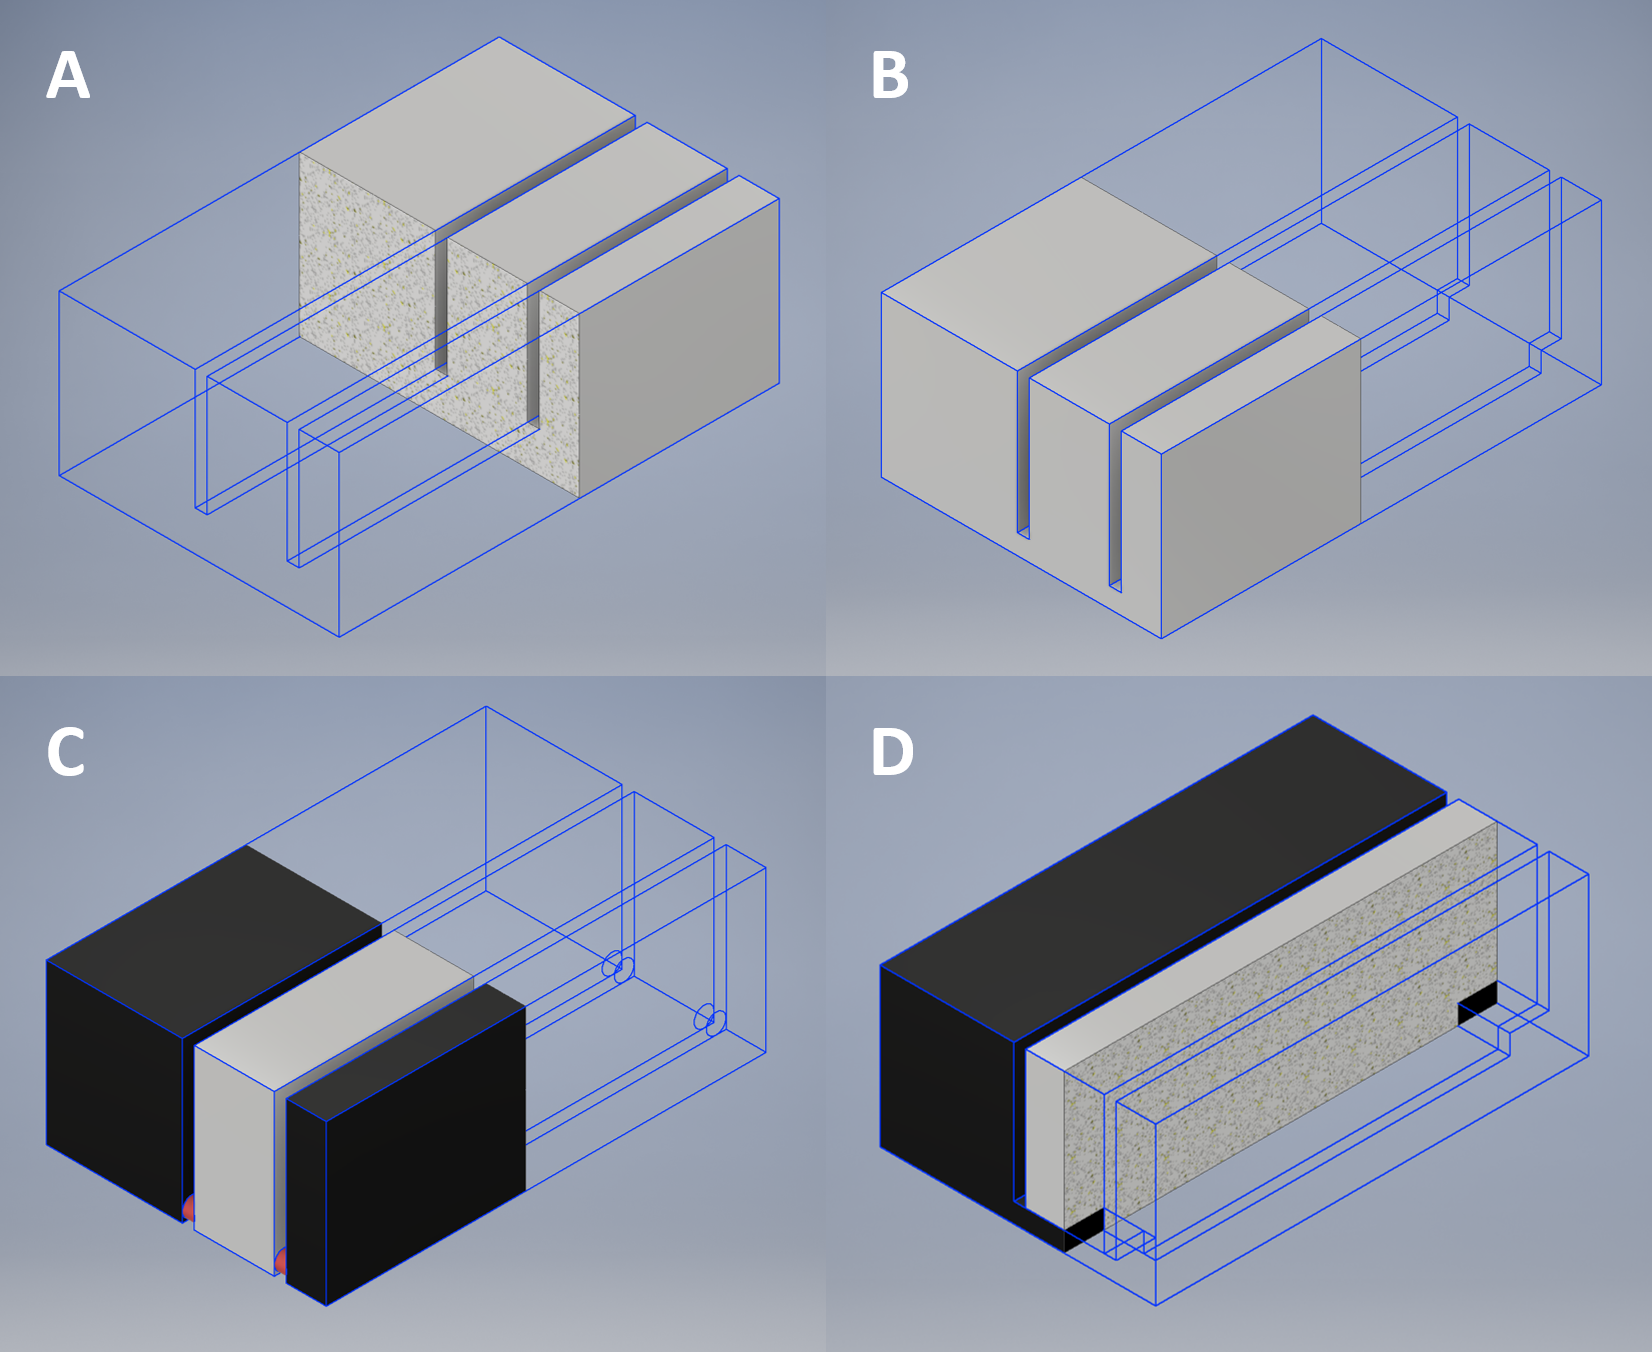
\includegraphics[width = \textwidth]{splitconcepts.png}
	\caption[Thermal Insulation Concepts.]{CAD representations of the thermal insulation concepts.}
	\label{fig:splitconcepts}
\end{figure}ˆ 
\FloatBarrier

Concept A features a groove machined into a solid billet of Aluminium, forming an air gap between the two regions. This concept has the advantage of simplicity, aiding with manufacture and serviceability. It's use of a single piece of material is also cost effective. It however had two main drawbacks. With the groove limited to a maximum of 3mm width and therefore 30mm deep, there is a large portion of material remaining which joins the two regions, leading to an undesirable level of heat transfer. Furthermore, the tooling costs involved with manufacturing this concept with the high aspect ration groove are significantly higher than with traditional machining operations. For these reasons, this concept required further development.\\

Concept B furthered the ideal behind Concept A by improving on some of its flaws, namely the transfer of heat. This was achieved by including further machining operations on the bottom face of the block. Therefore, the groove depth could be through the thickness of the block, apart from the small connecting regions on the outer edges of each groove. This simple change allowed the connecting area of material to be reduced to only 10\% of that of Concept A. Despite these improvements, the extra operations still require that small sections be machined at the same 30mm depth with the 3mm tool bit. Avoiding this is possible by performing machining operations on all four faces as opposed to only the top and bottom, however this will still carry added cost. Further to this, the homogeneous material and solid connection would allow for a more rapid heat transfer than was desirable. While aluminium is required for the Thermal Region due to its high level of heat transfer, this will result in large energy losses to the Carrier. It was therefore decided that the insulation should also make use of a thermally insulation material along with the physical separation used in the concepts to date.\\

Concept C moved in the direction of manufacturing the block from two separate materials and hence components. In Figure \ref{fig:splitconcepts}, Part C, the carrier is now seen to be of a different material, while the separating and insulating spacers are coloured in red. This allows the spacers to be manufactured from a highly insulating material, such as ethylene propylene as recommended by Williams et al. This concept provides excellent thermal insulation between the Thermal Region and the Carrier. The use of multiple parts however introduces another risk. The correct placement of the tubes in the Thermal Region is essential in ensuring the cassette tubes walls contact the heated block and hence the liquid is heated as required. One of the purposes of the carrier is to ensure the tubes are correctly located and positioned. With the carrier now manufactured from two separate parts and the Region being separate again, the alignment of all three parts has a considerable degree of flexibility. Therefore, ensuring all components are properly aligned and the tube contact occurs depends heavily on the fastening used and the assembly process itself. While possible to design an assembly method and fastening system that would locate the three components accurately, it was decided that this should be a feature of the design itself.\\

Concept D addressed these issues by using a single piece Carrier manufactured from a thermally insulating material. This was then designed so that the aluminium Thermal Region would sit directly inside a space machined from it. The use of this space meant that tolerances could be used to directly control the alignment of the Carrier and the Thermal Region and hence create a reliable tube fit to ensure consistent heating. In order to control the variation among the manufactured parts, the tolerance was set as a locational clearance fit. This fit provides a tight fit for locating the two parts, however under no circumstances allows interference and hence allows easy assembly and disassembly for servicing \cite{mmto}. The details of this fit are given in Table \ref{tab:fit}.

\begin{table}[h!]
\begin{center}
\begin{tabular}{ p{4.2cm} |  p{4.2cm} | p{4.2cm} }
\hline
Fit Classification & Minimum Clearance & Maximum Clearance\\ \hline \hline
Locational Clearance & 0.1mm & 0.2mm\\ \hline
\end{tabular}
\end{center}
\caption[Fit Tolerance Details.]{Details of Locational Clearance Fit.}
\label{tab:fit}
\end{table}

Due to the high degree of positional accuracy achieved by the fit described above, the design was able to be further simplified. Whether a TEC or resistive heaters were chosen, a heat sink was required on the bottom side of the device to fulfil the requirements of controller either heating device. This heat sink must be located on the bottom of the Thermal Region to extract thermal energy. Therefore, it may be used to "clamp" the single piece carrier and secure it in position. In this arrangement, the locational clearance fit locates the components in the X and Y directions, while the clamping force provided by securing the Thermal Region to the heat sink with the Carrier in between secures the Z direction movement. This allows a further reduction in hardware fasteners which not only increases manufacturability, but also reduces heat transfer due to conductive transfers that are created by fasteners such as bolts.

\subsubsection{Heater Selection}
\label{sec:heaterselection}

In order to achieve the heating requirements of the extraction process, two main heating devices were considered, as were explored in Chapter \ref{cha:literaturereview}, Literature Review. These were the solid state TEC and the resistive heat strip.\\

After consideration of the properties of each device, the TEC was selected as the heating device to be used. While the resistive heating elements are cost effective, easily installed, possess a long service life and can generate large quantities of thermal energy, the TEC has a number of significant advantages. The TEC modules are a solid state device and hence provide a highly reliable means of thermal management. The devices, provided they are installed correctly, may last for up to 200,000 hours of use \cite{Ferroteclife}. This figure is supplied by Ferrotec, the supplier of TEC's used by AusDiagnostics, and is stated to be an accepted industry standard MTBF (Mean Time Between Failures). Along with this high level of reliability, these modules are capable of provide precise temperature control to within $\pm$ 0.1$\degree$C. This advantage is paired with their simple power supply requirements, being able to be controlled via PWM (Pulse Width Modulation) directly from a DC power source. The TEC devices available are also capable of outputting significant amounts of thermal energy, with single state devices able to transfer up to 6 $W/cm^2$ of device surface area \cite{Ferroteclife}. By far the greatest advantage however, is the ability of the TEC to pump heat in either direction to enable both heating or cooling of the target component with the same installing. As was described in Chapter \ref{cha:literaturereview}, Literature Review, this is controlled simply by inverting the direction in which current is applied to the terminals of the TEC. This has large significance for the control of the system temperature, as the controller can actively drive the temperature in the necessary direction to drive the error to 0, as opposed to relying purely on passive methods or even fan based cooling.\\

With the device to be used now selected, the power requirements of the TEC needed to be determined. In order to ensure the selected TEC would be capable of driving the temperature of the Thermal Region to 60$\degree$C, the thermal transfers of the system needed to be understood. As the Thermal Region reaches is target temperature, losses will begin to occur at a greater rate to its surroundings due to the increasing temperature differential. The power of this energy transfer must be at the very least matched by the power output of the TEC to maintain a stable temperature, or exceeded to drive the temperature change at an acceptable rate. To determine these variables, a number of design parameters are required:
\begin{enumerate}
	\item [$T_h$] This is the maximum hot side temperature of the TEC module. For this application, the module will need to drive the Thermal Region to 60$\degree$C and therefore this temperature is selected. However, it is recommended that for large thermal loads, or those were the path of heat transfer is greater than 25mm, that this variable be increased by 5$\degree$C. This application involves both of these conditions and therefore:
	$$T_h = 65\degree C$$
	\item[$T_c$] This variable is determined by the minimum expected ambient temperature in which the device will work within along with the capacity of the applied heat sink. If the system operates with a small thermal load and adequate heat sinking, then the following equations is applied:
	\begin{equation}
	T_c = T_{ambient} - 5\degree C
	\end{equation}
	However, for a system with a large thermal load and a small level of heat sinking, the following is substituted:
	\begin{equation}
	\label{eq_tc}
	T_c = T_{ambient} - 15\degree C
	\end{equation}
	With the device matching the conditions of a large thermal load with small heat sinking, Equation \ref{eq_tc} is applied. Given that the Gene-Plex Extractor will operate within enclosed indoor facilities, 20$\degree$C was selected as the minimum expected ambient temperature. Therefore,
	$$ T_c = 20 - 15$$
	$$ T_c = 5\degree C $$
\end{enumerate}

In order to calculate the thermal load which the TEC's must displace to drive a temperature change, the various thermal transfers of the system must be estimated. These loads may be split into active and passive loads:
\begin{equation}
\label{eq_thermalload}
Q = Q_{active} + Q_{passive}
\end{equation}

\begin{enumerate}
	\item [Active] These loads are due to the power dissipated by the device as part of the electrical components. In the case of the Processor Module, this load is negligible due to the significant separation between the electronics and the thermally controlled elements:
	$$Q_{active} = I^2R = 0 $$ 
	\item[Passive] These loads are those due to heat transfers within the device and to its surroundings. These consist of radiation, convection and conduction:
	\begin{equation}
	\label{eq_passive}
	Q_{passive} = Q_{radiation} + Q_{convection} + Q_{conduction}
	\end{equation}
	
	Radiative thermal transfers are found using:
	\begin{equation}
	\label{eq_rad}
	Q_{radiation} = F\epsilon\sigma A(T_h^4 - T_c^4)
	\end{equation} 	
	where,\\
	F = Shape Factor = 1 (assume worst case scenario)\\
	$\epsilon$ = Emmisivity = 1 (assume worst case scenario)\\
	$\sigma$ = Stefan-Boltzman Constant = $5.667\times10^{-8} W/m^2K^4$\\
	A = Surface Area $(m^2)$\\
	$T_h$ = Maximum TEC hot side temperature (K)\\
	$T_c$ =  Minimum TEC cold side temperature (K)\\
	
	Convective thermal transfers are found using:
	\begin{equation}
	\label{eq_cov}
	Q_{convection} = hA(T_h - T_c)
	\end{equation} 	
	where,\\
	h = Convective heat transfer coefficient = 21.7 $W/m^2$ $\degree$C\\
	$\epsilon$ = Emmisivity = 1 (assume worst case scenario)\\
	$\sigma$ = Stefan-Boltzman Constant = $5.667\times10^{-8} W/m^2K^4$\\
	A = Surface Area $(m^2)$\\
	$T_h$ = Maximum TEC hot side temperature (K)\\
	$T_c$ = Minimum TEC cold side temperature (K)\\

	Conductive thermal transfers are found using:
	\begin{equation}
	\label{eq_cond}
	Q_{conductive} = \frac{KW}{L}(T_h - T_c)
	\end{equation} 	
	where,\\
	K = Thermal Conductivity of material ($W/m$ $\degree$C)\\
	W = Cross sectional area of material ($m^2$)\\
	L = Length of thermal transfer path (m)\\
	 
\end{enumerate}

Using these equations, the thermal load of the Thermal Region was determined to be:
$$ Q \approx 47 W $$

This figure was determined using the equations discussed via a MATLAB script. For this estimation, some simplifications were made. This includes neglecting the effects of radiative loads due to their low weighting in this result. Furthermore, only the significant bodies and thermal transfers in the assembly were modelled. The purpose of obtaining this estimate was to guide a good starting point for TEC selection. Comprehensive CFD was completed as a later step, as detailed below, and therefore a high level of accuracy was not necessary in this calculation.\\

Using this figure and comparing the available TEC modules available from suppliers, it was decided that this power requirement could be most effectively met by utilizing 3 TEC's, each with a 16W capacity. This divide matches closely with the available module power outputs when considering the area to which they will be mounted, as achieving this output from a single device would result in a module that exceeds the area available for mounting.\\
	
The maximum temperature differential expected in this application is $\Delta T = T_h - T_c = 60\degree$C. This is comfortably within the 72$\degree$C $\Delta$T limit of a single stage TEC. Therefore, single-stage modules will be used.\\

The modules selected for use were the Ferrotec 9500-035-085 B. The device has dimensions 15.1mm (W) $\times$ 29.8mm (L) $\times$ 3.94mm (H). It's performance values are summarised in Table \ref{tab:TECspec}. This module can be seen to exceed the thermal power requirement by a comfortable margin of 4 Watts.

\begin{table}[h!]
	\begin{center}
		\begin{tabular}{ p{3.15cm} |  p{3.15cm} | p{3.15cm} | p{3.15cm } }
			\hline
			I Max & V Max & $\Delta$T Max & $Q_c$ Max\\ \hline \hline
			8.5 A & 4.8 V & 72 $\degree$C & 22.0 W\\ \hline
		\end{tabular}
	\end{center}
	\caption[Ferrotec 9500-035-085 B Performance Specifications.]{Ferrotec 9500-035-085 B Performance Specifications.}
	\label{tab:TECspec}
\end{table}

\subsubsection{CFD Simulation - Initial Design}
\label{initialcfd}

With the TEC modules selected, the module's design was completed in Autodesk Inventor Professional to enable CFD Simulation to be completed. This first stage of CFD was used gauge the first design iterations ability to heat the Thermal Region to the desired set temperature.\\

To ensure the efficient usage of computing resources, the design was simplified appropriately with the following changes made:
\begin{itemize}
	\item Removal of all corner fillets and chamfers.
	\item Removal of interferences between components, such as where foam insulators will be compressed.
	\item Detailed TEC module component replaced with simplified rectangular prism.
	\item Bolted connection and associated holes removed.
	\item Circuit board removed.
\end{itemize}

These simplifications allowed for the model to be meshed with a total of $2.1\times 10^6$ elements.

While the specifics of the CFD setup are not presented, it is noted that the Chimney approach was used for the boundary condition setup. This setup is applied to the body of air surrounding the model. This body of air then has two boundary conditions applied. The first is a 25$\degree$C temperature boundary condition on the bottom face. This is then completed with two 0 kPa pressure boundary conditions on the top and bottom faces. With this setup, the simulation was run to convergence.\\

\subsubsection{Discussion}

The simulation conducted provided a number of key results. These include the adequate performance of the TEC modules and setup selected, evidence to support reducing the number of TEC modules used in each Processor Module and finally, possible areas in which the mechanical design can be improved.\\

A study of the cross sectional temperature gradient throughout the Thermal Region displayed a high level of consistency across the component and therefore validated the mechanical design.

The simulation also demonstrated the TEC modules were operating at a very high Coefficient of Performance (COP). It should be noted that is in fact possible to operate at COP's of greater than 1, as this value is obtained by the equation \cite{Ferroteceff}:
\begin{equation}
COP = \frac{Q_h}{P_{in}}
\end{equation}
where,

$$Q_h$$ is the thermal power generated by the TEC at the hot side.\\
$$P_{in}$$ is the power supplied to the TEC.\\

The COP obtained in this simulation suggests the TEC's are operating below their maximum operating point in order to drive the Thermal Region to this temperature. This was further shown by the maximum current value, which demonstrated the module operating at less than 10\% of it's maximum, as was given in Table \ref{tab:TECspec}. While operating at a fraction of $I_{max}$ gives a higher efficiency, there are advantages of operating at a point nearer this value. Due to the Ferrotec TEC modules costing around \$16.00 each, reducing the number of TEC's per Processor Module is advantageous due to the cost reduction this would achieve for each Gene-Plex Extractor.\\

Finally, the results of this initial simulation identified an area through which significant heat transfer was occurring and must be reduced. This region was found to be at the meeting plane of the Thermal Region and the Carrier, where an overlap between the two parts was created along the entire perimeter of the Thermal Region. This design feature was used to ensure a level placement and proper location of the Thermal Region with respect to the Carrier. However, the area of material used to achieve this may be reduced significantly to avoid the thermal losses occurring as a result.\\

\subsubsection{CFD Simulation - Refined Design}
\label{refinedcfd}

The results drawn from the initial experiment were then applied to form a refined design. This section described the results obtained from the analysis of this design. The two major refinements made include the reduction of TEC modules from three to two, along with the reduction in contact area between the Thermal Region and the Carrier.\\

The refined design was then simulated using an identical setup as was used previously. The results of this simulation, after the solver had reached convergence, are given in Figure \ref{fig:result2}. Once again, the convergence plot for this simulation is provided in Appendix \ref{cha:CFDconverg}.

\begin{figure}[!htb]
	\centering
	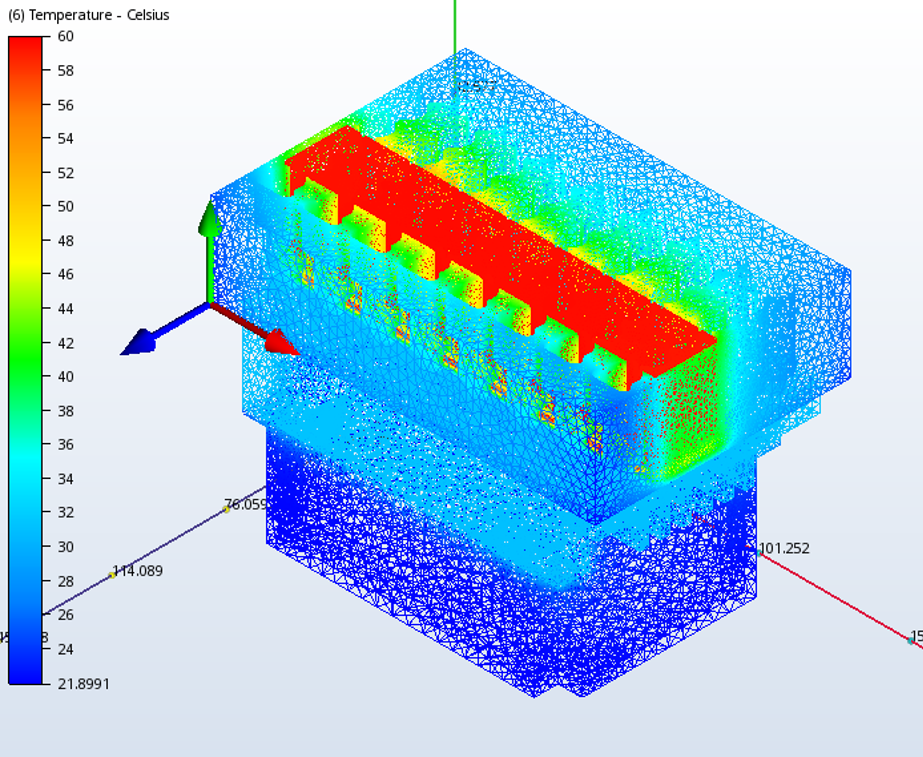
\includegraphics[width = \textwidth]{result2.png}
	\caption[CFD Results - Refined Design.]{Final results of the CFD Simulation of the refined design.}
	\label{fig:result2}
\end{figure}ˆ 
\FloatBarrier

Figures \ref{fig:cutcfd} below show the temperature variation across the Thermal Region normal to the X, Y and Z axes.

\begin{figure}[!htb]
	\centering
	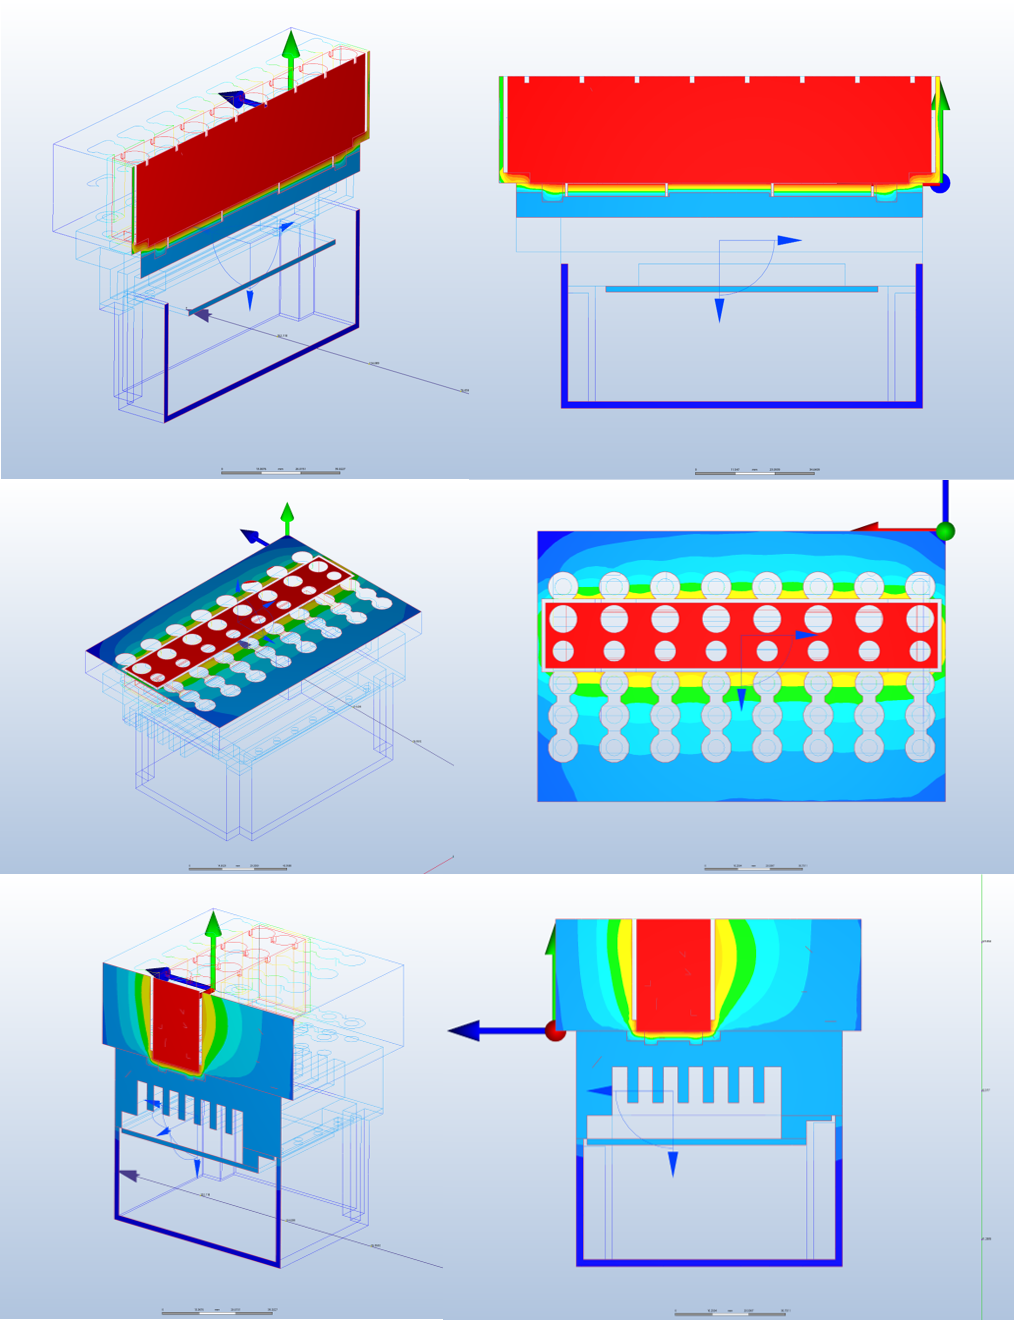
\includegraphics[width = \textwidth]{cutcfd.png}
	\caption[CFD Results - Spatial Variations of Temperation.]{Spatial variation of temperature through the XY, XZ and YZ planes of the Thermal Region.}
	\label{fig:cutcfd}
\end{figure}ˆ 
\FloatBarrier

The thermal transfer between the Thermal Region and the Carrier are shown along the YZ plane in Figure \ref{fig:thermalvariation}.

\begin{figure}[!htb]
	\centering
	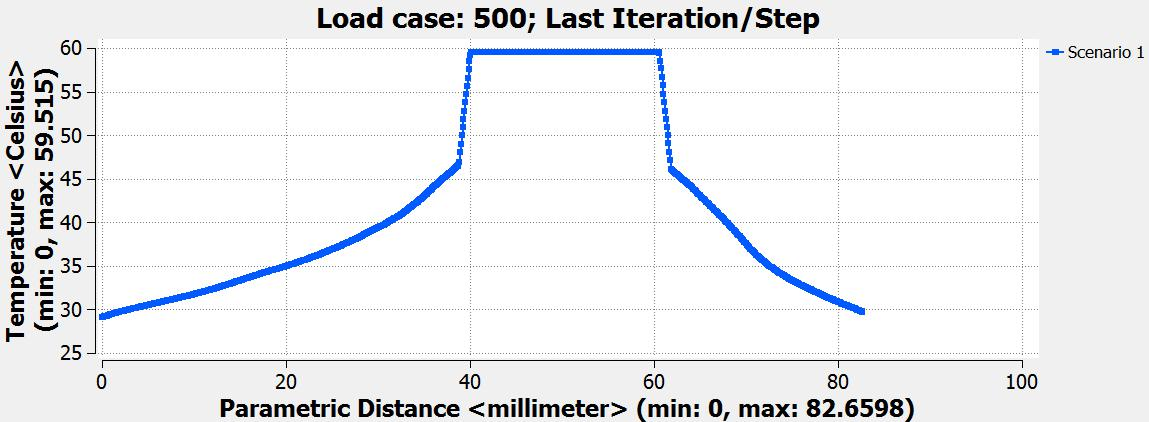
\includegraphics[width = \textwidth]{thermalvariation.jpg}
	\caption[CFD Results - Thermal Losses from Thermal Region to Carrier.]{Thermal Losses from Thermal Region to Carrier.}
	\label{fig:thermalvariation}
\end{figure}ˆ 
\FloatBarrier

The critical TEC performance values are summarised below in Table \ref{tab:TECperf2}:

\begin{table}[h!]
	\begin{center}
		\begin{tabular}{ p{5.15cm} |  p{3.15cm} | p{3.15cm} }
			\hline
			TEC No. & 1 & 2 \\ \hline
			Status A & Normal & Normal \\ \hline
			Cold Side Temperature & 31.00 $\degree$C & 31.25 $\degree$C \\ \hline
			Hot Side Temperature & 60.00 $\degree$C & 60.00 $\degree$C \\ \hline
			Power Input & 3.53 W & 3.37 W \\ \hline
			Operating Current & 1.43 A & 1.40 A \\ \hline
			COP & 0.92 & 0.94 \\ \hline
		\end{tabular}
	\end{center}
	\caption[Ferrotec 9500-035-085 B Simulated Performance.]{Ferrotec 9500-035-085 B Simulated Performance.}
	\label{tab:TECperf2}
\end{table}

\subsubsection{Discussion}

By comparison between the results obtained by simulating the refined design as opposed to the initial design and by analysing the critical data points, a number of key points may be noted.\\

Most critically, the sectioned views in Figures \ref{fig:cutcfd} show a consistent temperature distribution is still attained despite the drop to two TEC modules. The results show an average temperature across the Thermal Region of 59.58$\degree$C, and a minimum temperature of 58.78$\degree$C. The results validate the performance of the hardware design in providing a stable platform for temperature control to be carried out within.\\

Considering the performance figures of each of the TEC modules in Table \ref{tab:TECperf2}, the suitability of the reduction in TEC units can be assessed. Given the minimum COP of 0.92 and the maximum operating current of 1.43 A resulting in a 16.8\% usage of each devices operating limit, the modules are shown to be working within their operating limits at a high efficiency when holding the Thermal Region at a steady state 60$\degree$C.\\

As a result of the experiment conducted, the configuration simulated is seen to achieve the stipulated operating requirements as well as make effective use of the capabilities of the heating components. Therefore, this configuration is selected as the final design for the Processor Module.

\subsection{Final Mechanical Design}
\label{sec:mechdesign}

With the mechanical design validated by a thorough CFD simulation and analysis, the final design was determined and finalised. The following is a summary of the notable features of the result of this process.\\

Due to the results of the intial simulations in Section \ref{initialcfd} and the validation obtained in Section \ref{refinedcfd}, the method of locating the Carrier on the Thermal Region was revised. The result is the locating design displayed in Figure \ref{fig:carrierlocation}, where a small overlap of the Thermal Region on the Carrier is used to lock the Carrier between the Thermal Region and the heak sink it is fastened to. This design choice allows the Carrier to be held in place with no fasteners. As was discussed in Section \ref{sec:isolation}, this will constrain only the movement in the Z direction. Therefore, the locational clearance fit of Concept D is used to ensure complete location of the Carrier, without the direct use of a fastener.

\begin{figure}[!htb]
	\centering
	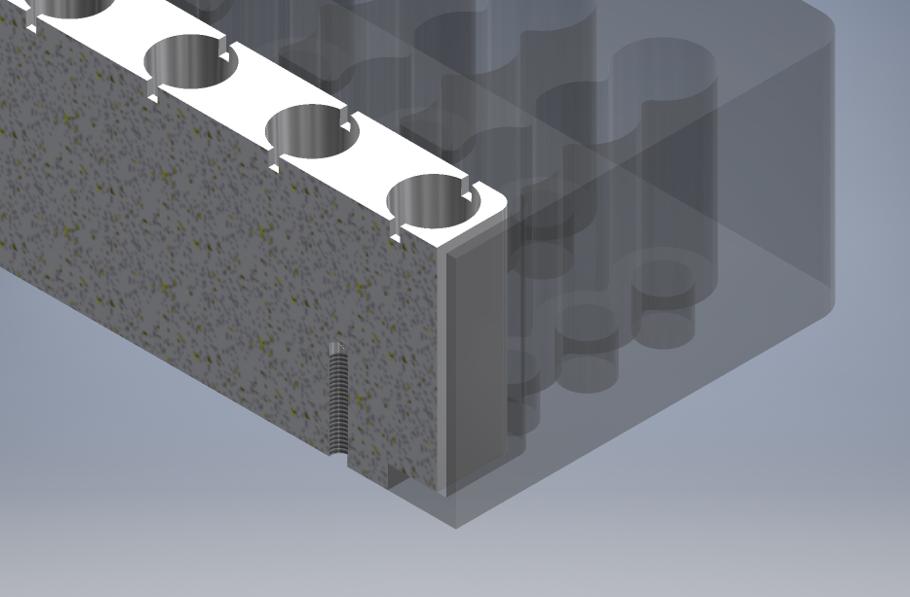
\includegraphics[width = \textwidth]{carrierlocation.png}
	\caption[Design for Carrier Location on Thermal Region.]{Design for accurate carrier location around the Thermal Region.}
	\label{fig:carrierlocation}
\end{figure}ˆ 
\FloatBarrier

The design of the Carrier itself was considered to ensure it fulfils two main purposes. These are prevention of user contact with the hot Thermal Region and ensuring the correct positioning of the cassette tubes in the Thermal Region. The first purpose is to ensure the design complies with Standard BS EN 61010-1:2010 \cite{BSI} in preventing the user from unintentionally making contact with the hot component during normal operation. The combination of the Carrier and the installed cassette tubes provide full coverage of the Thermal Region and hence prevent such contact occurring unintentionally. Finally, the design of the Carrier is such that it does not allow the cassette tubes to be misplaced by the user. This is achieved via a number of design elements. Firstly, the Carrier itself prevents the cassette tubes from being positioned in the Processor Module in the reverse orientation. The fit of the cassette tubes in the Thermal Region is then controlled by the geometry of the tube holes in the Carrier wells. As is pictured in Figure \ref{fig:carrierfit}, the cassette tubes are tightly fitted within the Thermal Region, while sitting in the Carrier supported only at their base to control their height. This ensures that the fit within the Thermal Region is accurate independent of the manner in which the user places the tubes into the Processor Module, by preventing rocking. Furthermore, it ensures any deviation of the Carrier's position around the Thermal Region due to the locational clearance fit does not force the cassette tubes out of contact with the heated material.

\begin{figure}[!htb]
	\centering
	\includegraphics[width = \textwidth]{carrierfit.png}
	\caption[Cassette tube fit within Carrier and Thermal Region.]{Cassette tube fit within Carrier and Thermal Region ensures a reliable contact on the heated tubes.}
	\label{fig:carrierfit}
\end{figure}ˆ 
\FloatBarrier

The heat sink designed for the Processor Module is required to maintain the stable thermal state during both heating and steady state operation. As was noted in Chapter \ref{cha:literaturereview}, Literature Review and in Section \ref{sec:heaterselection}, the TEC modules will only pump heat if they are operating below a $\Delta$T of 72$\degree$C. the design parameter set was to maintain the heat sink at a maximum of 15$\degree$C below ambient. It was decided to achieve this via passive cooling of the heat sink using only natural transfers, as opposed to an active approach using a fan, for example. This was to reduce overall system complexity, system power requirements and cost of each Processor Module. Therefore, it was necessary to ensure the heat sink comprised of a large thermal mass and surface area to promote heat transfers with the surrounding air and to ensure a slow rate of response to the heat energy that the TEC modules will introduce.\\

Further to this, the heat sink is used as the mounting location for the TEC modules and the associated wires and sensors. The final design of the heat sink is pictured in Figure \ref{fig:heatsink}, with the two TEC's. The insulator and the TEC Spacers shown in grey and black respectively.

\begin{figure}[!htb]
	\centering
	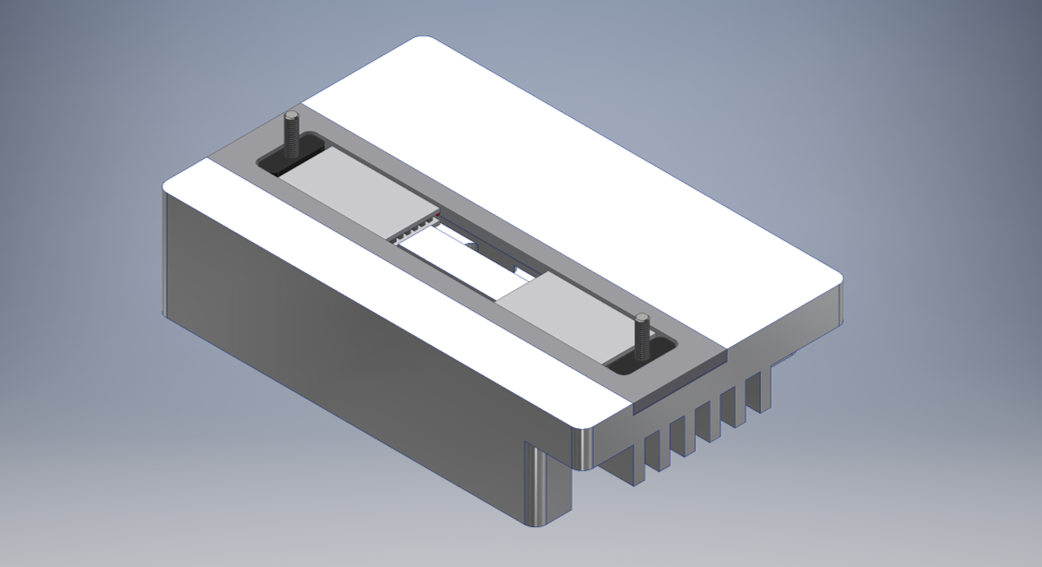
\includegraphics[width = \textwidth]{heatsink.png}
	\caption[Heat sink final design.]{The final heat sink design, including TEC housing and wire and sensor accommodation}
	\label{fig:heatsink}
\end{figure}ˆ 
\FloatBarrier

The insulator placed around the perimeter of the TEC modules is a critical design feature. It ensures that the heated and cooled regions fo the Thermal Region and heat sink respectively are not able to transfer heat energy via conduction to one another, and forms the separating piece between both components. The insulator is made of a silicon gasket insulator \cite{jehbco}, and has been proven effective as an insulator in the AusDiagnostics MTX Cycler. Further to this, the silicon material used has a surface skin that results in a very low absorption of liquid \cite{jehbco}. This feature has allowed the insulator to form a seal around the open areas of the design, to ensure no split liquid or chemicals are able to enter the internal device area.\\

The TEC Spacers are two components placed around the bolted connections, shown in black. These components are included in order to ensure the operation life of the TEC modules is not compromised by uneven loading. Due to the asymmetrical design of the heat sink, it is possible that an uneven load may result across the face of the TEC modules. It is also critical that the modules are clamped between an evenly spaced void to reduce as much as is possible any shear loading. The Acetal TEC Spacers achieve this by ensuring the heat sink and Thermal Region are parallel when assembled, while also ensuring the spacing between the TEC surfaces is consistent. The components are machined from Acetall, due to its properties as a good insulator, good thermal stability and the high accuracy with which it may be machined.

In order to ensure the TEC modules are then adequately clamped and are in ideal conditions, the two fastening bolts must be torqued precisely. The recommendation provided by Ferrotec, the TEC manufacturer, is as follows:
\begin{equation}
\tau = \frac{S_a A}{N}Kd
\end{equation}
where,
\begin{itemize}
	\item $S_a$ is given as 25-50 psi for a cycling application, or 50-75 psi for static applications such as this.
	\item A is the total surface area of the TEC modules.
	\item N is the number of bolts used to clamp the modules.
	\item K is the torque coefficient, recommended as 0.2 for steel fasteners.
	\item d is the nominal bolt diameter. In this case, two M3 bolts are used and hence $d=3$.
\end{itemize}
Therefore:
$$\tau = \frac{(3444738 pa)(9\times 10^{-4}m^2)}{2}(0.2)(3\times10^{-3}m)$$
$$\tau = 0.93 Nm$$

A fully exploded rendering of the final Processor Module design is given in Figure \ref{fig:exploded}.

\begin{figure}[!htb]
	\centering
	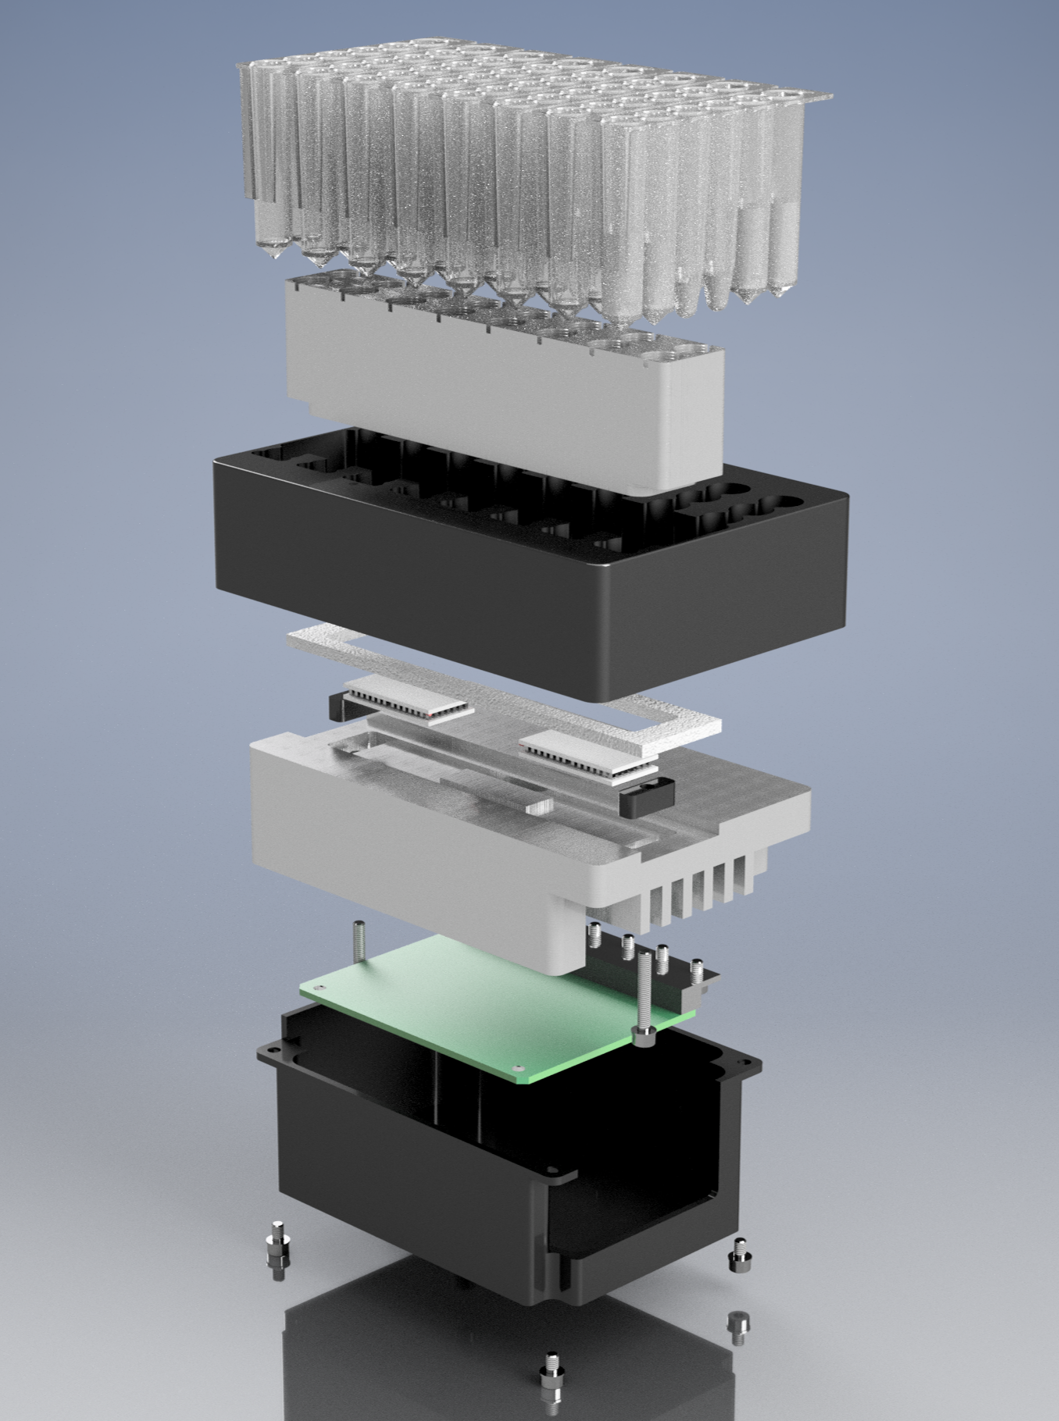
\includegraphics[width = \textwidth]{exploded.png}
	\caption[Processor Module Exploded Rendering.]{An exploded representation of the final Processor Module Design.}
	\label{fig:exploded}
\end{figure}ˆ 
\FloatBarrier

\subsection{Processor Module Assembly}

This section provides a brief and summarised overview of the assembly process of one of the 10 Processor Modules which were manufactured following the design and validation completed. This work is completed in preparation for the controller design, detailed in Section \ref{sec:ControllerDesign}. The full set of manufactured components are pictured in Figure \ref{fig:1}, and includes (from left to right) the:
\begin{itemize}
	\item Carrier
	\item Heat sink
	\item TEC Spacers
	\item Thermal Region
	\item Ferrotec TEC Modules
	\item TEC Gasket/Insulator
\end{itemize}

\begin{figure}[!htb]
	\centering
	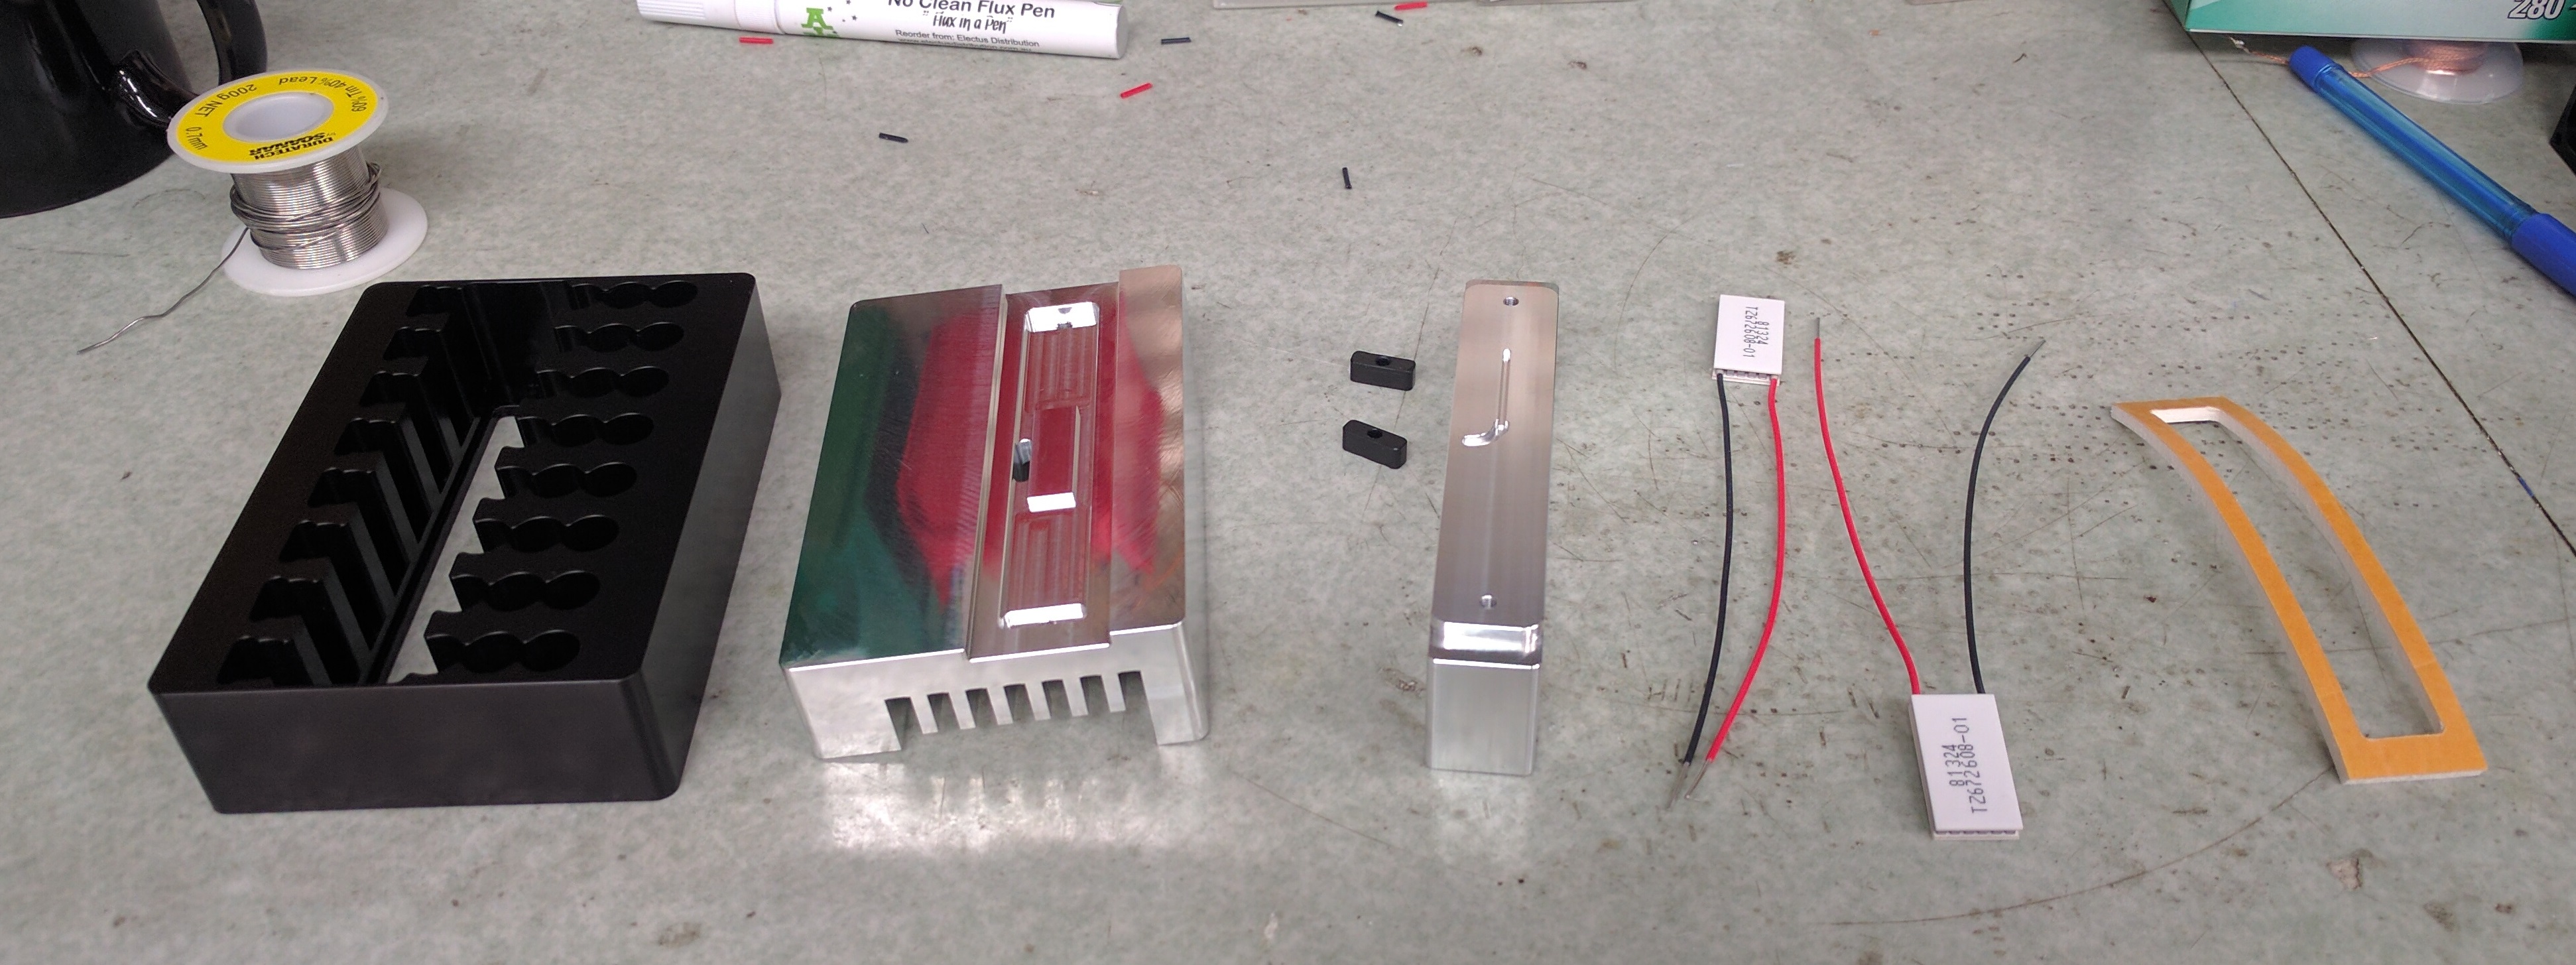
\includegraphics[width = \textwidth]{1.jpg}
	\caption[Processor Module Components.]{All Processor Module components (MTX Cycler electronics board not included).}
	\label{fig:1}
\end{figure}ˆ 
\FloatBarrier

The first stage is to prepare the two TEC modules to be used within the assembly, as shown in Figure \ref{fig:2}. This required wiring and soldering the modules in series and protecting the connections to ensure reliable operation.

\begin{figure}[!htb]
	\centering
	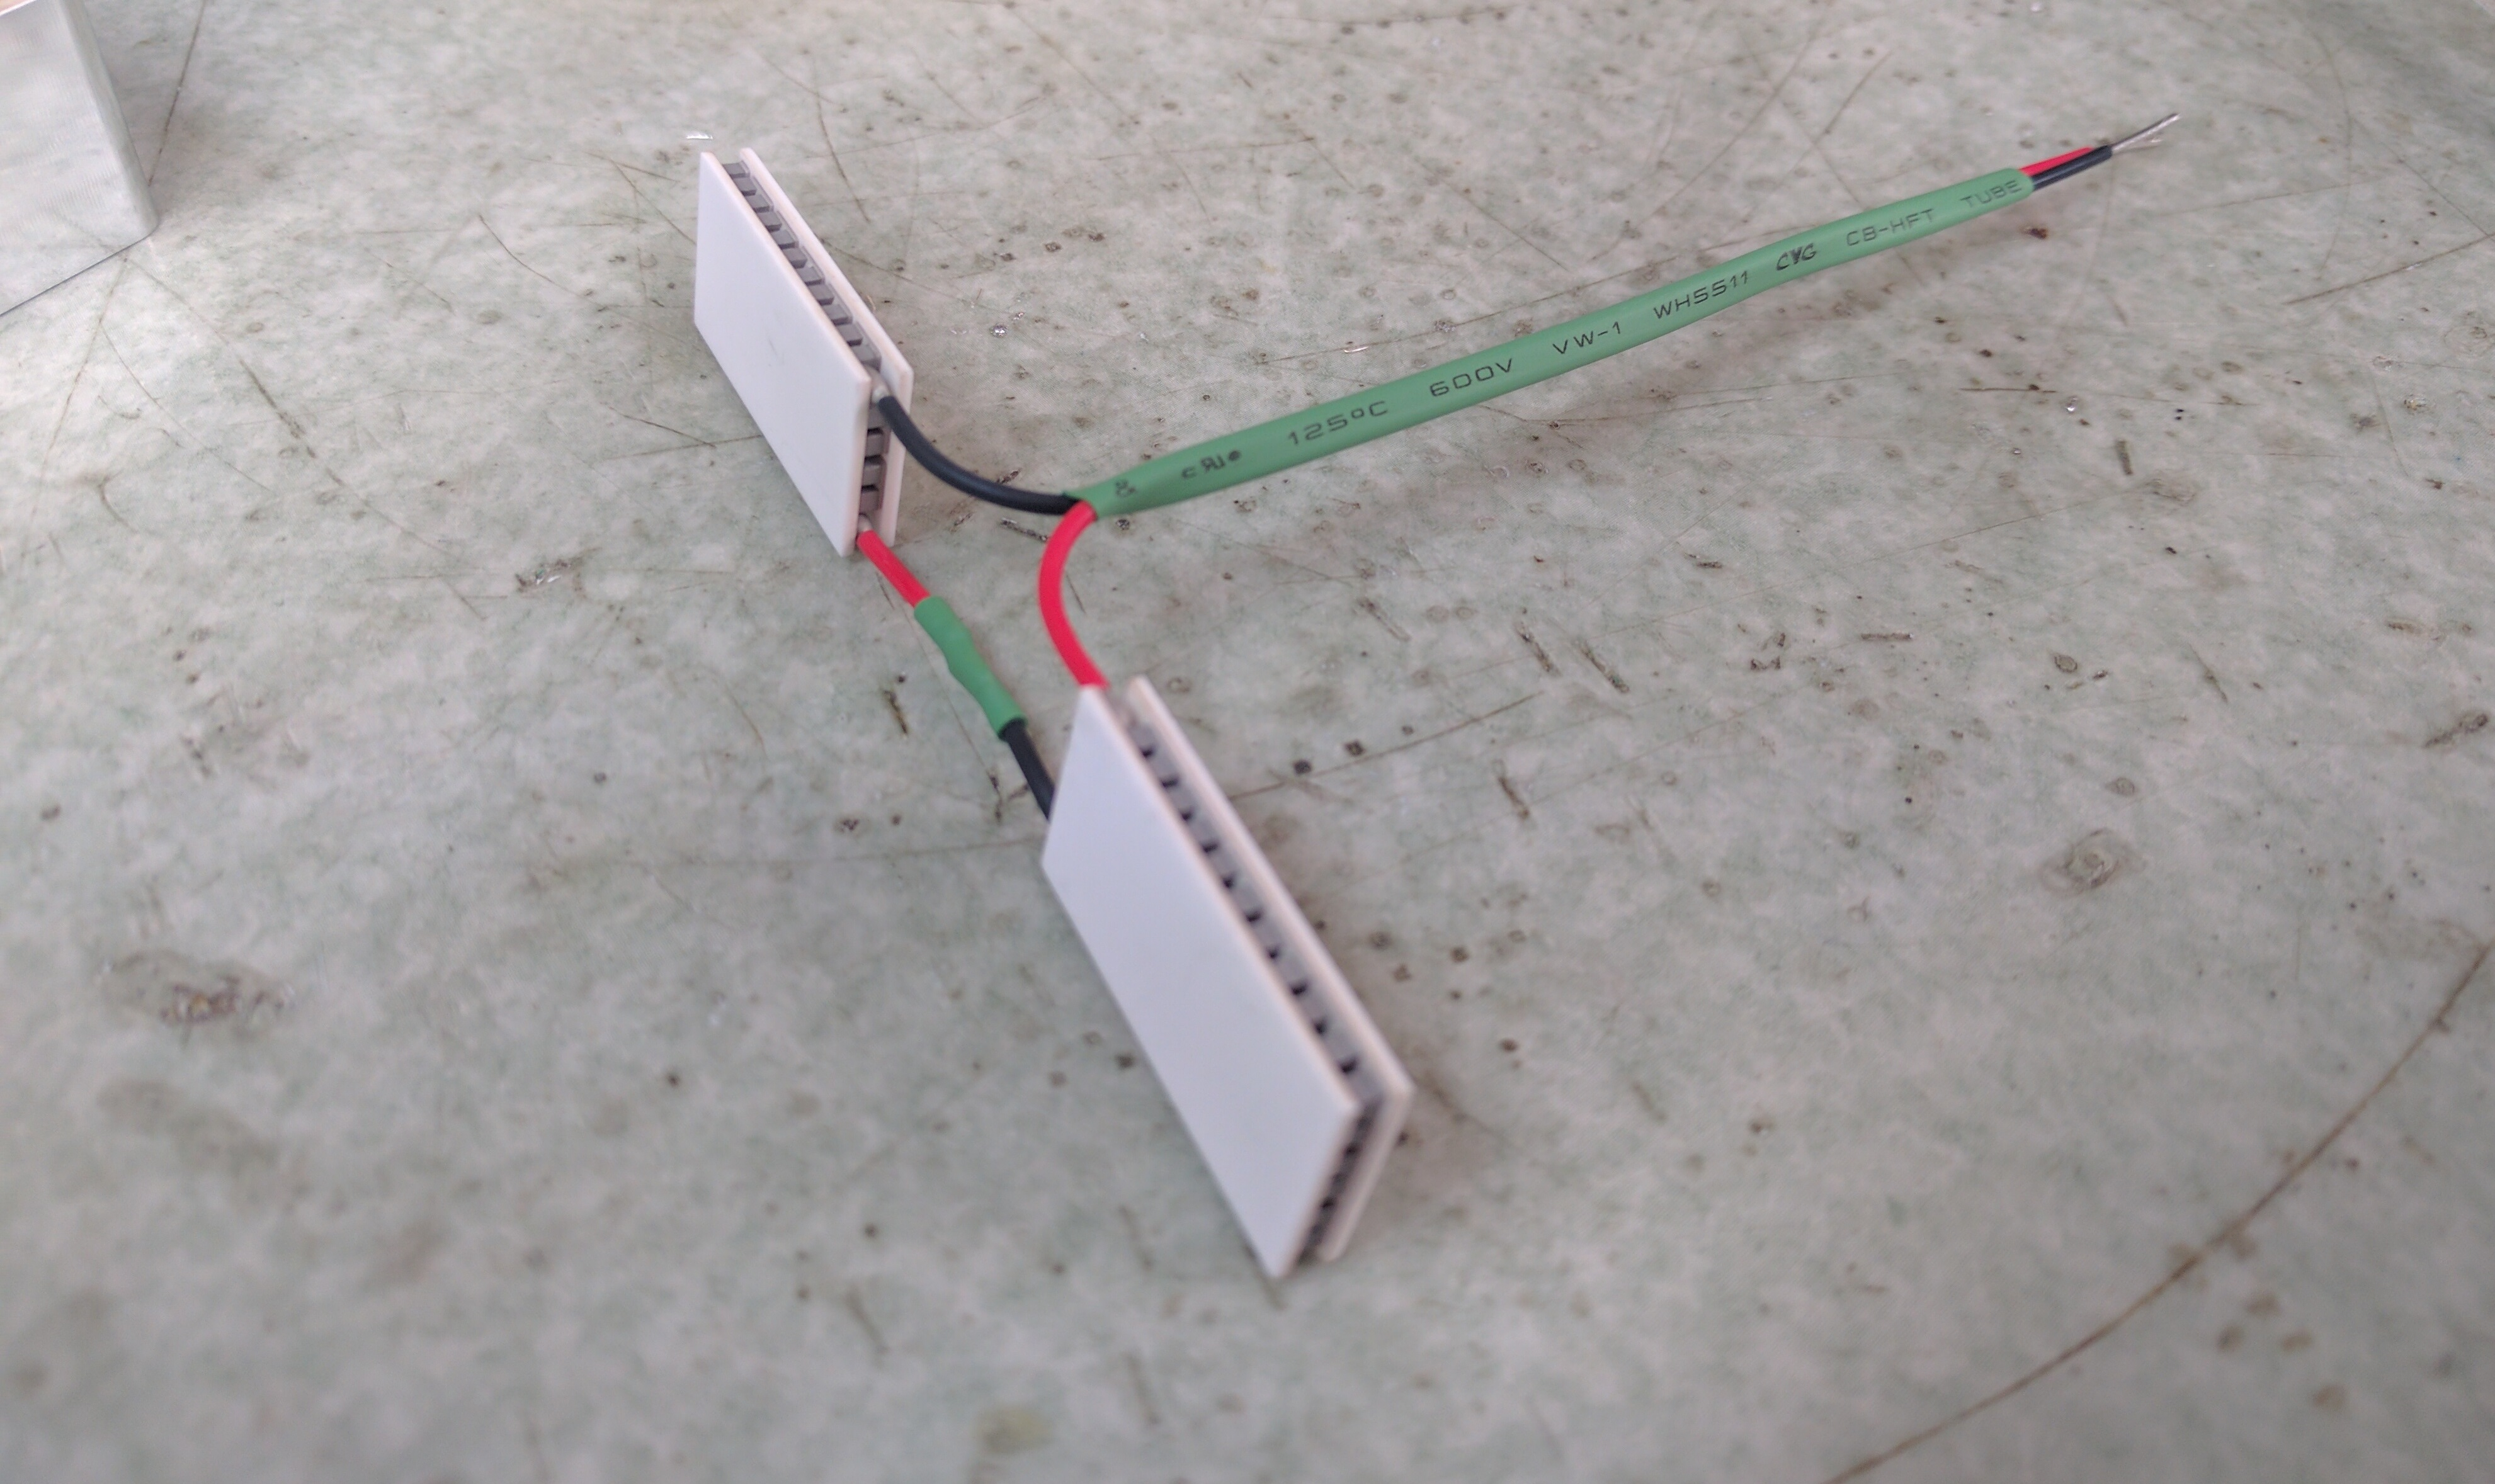
\includegraphics[width = \textwidth]{2.jpg}
	\caption[TEC Module connection.]{The assembly of the Processor Module's two TEC modules.}
	\label{fig:2}
\end{figure}ˆ 
\FloatBarrier

Prior to placement in the heat sink, it is crucial that a thermally conductive paste is applied evenly to the surface as in Figure \ref{fig:3}. The thickness of this coating must be 0.02mm or less, however ensures full contact is made between the TEC and the surface along with providing necessary lubrication for the expansion experienced by the device.

\begin{figure}[!htb]
	\centering
	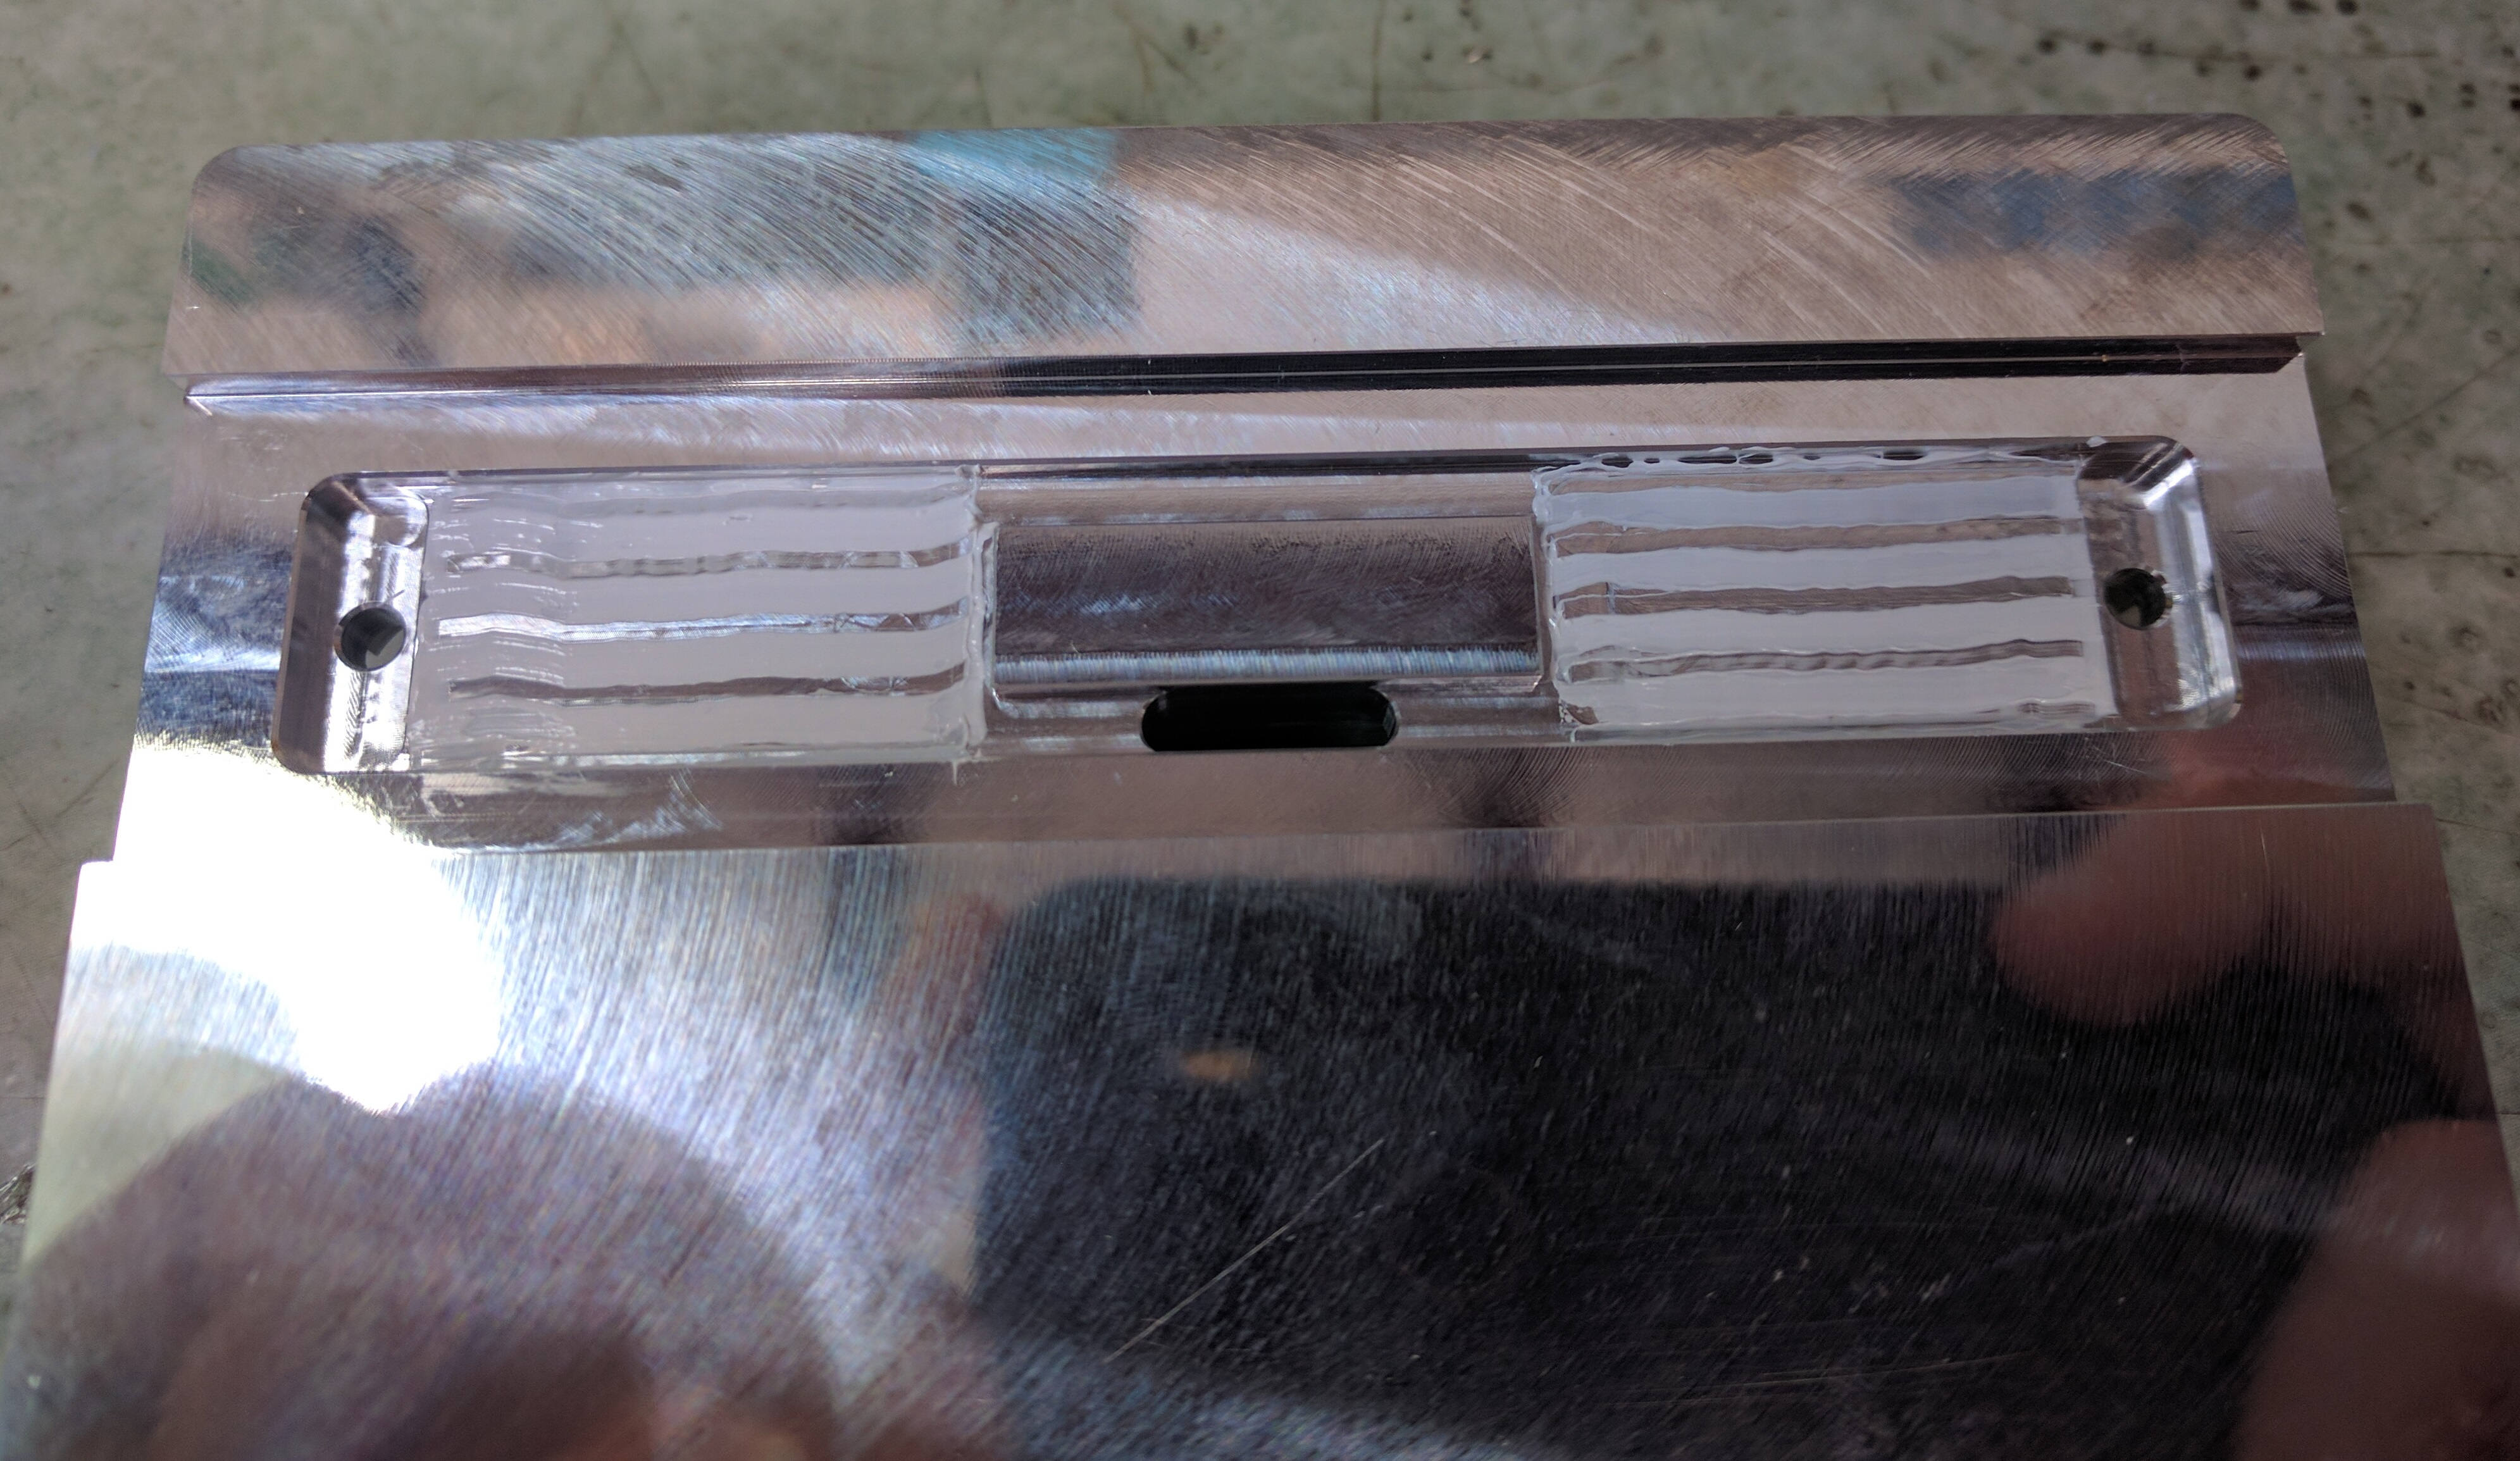
\includegraphics[width = \textwidth]{3.jpg}
	\caption[Heat sink thermal paste application.]{Application of thermally conductive paste to the contact area of the TEC modules.}
	\label{fig:3}
\end{figure}ˆ 
\FloatBarrier

Following this, the TEC's may be placed into the heat sink and their wiring directed through the port. The TEC Spacers and the insulator/gasket is also attached via its adhesive backing to the heat sink. A final identical layer of thermal paste is once again required on the hot side of the TEC modules. This stage is shown in Figure \ref{fig:4}.

\begin{figure}[!htb]
	\centering
	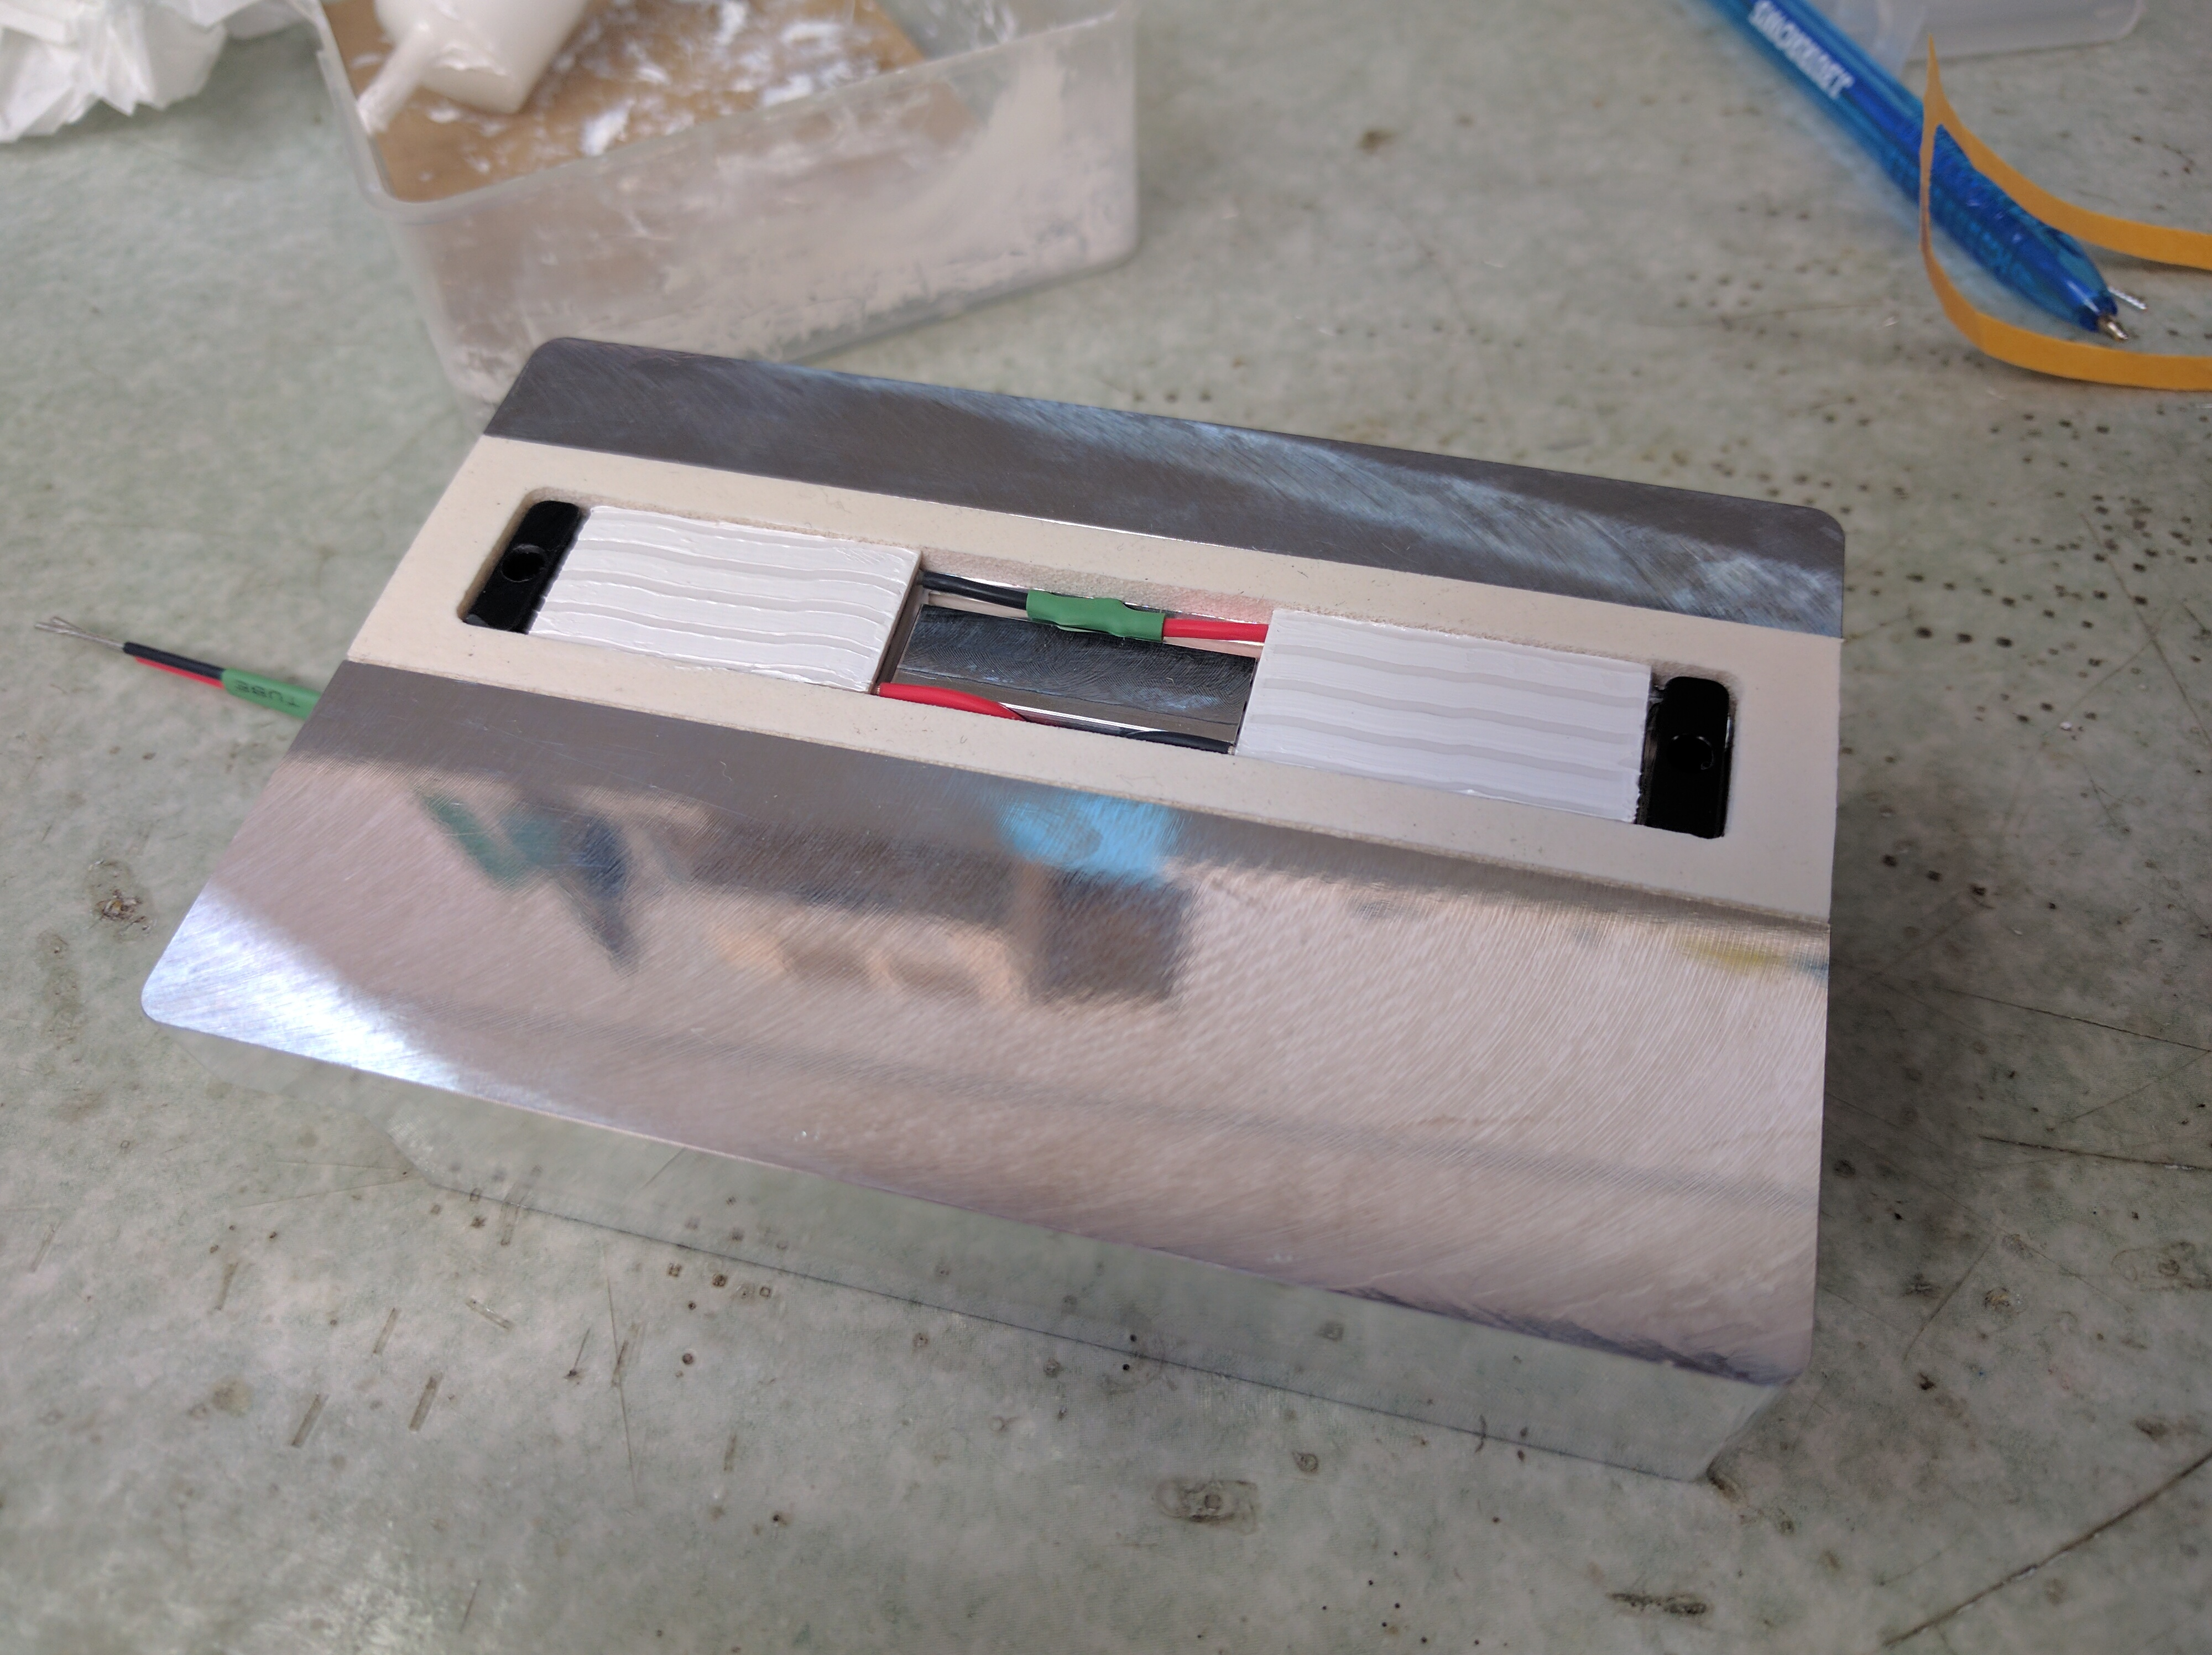
\includegraphics[width = \textwidth]{4.jpg}
	\caption[Heat sink component assembly.]{Placement of the TEC modules, gasket/insulator and TEC spacers into the heat sink.}
	\label{fig:4}
\end{figure}ˆ 
\FloatBarrier

Before final positioning, the required wiring is added to the thermistor sensor and protected, as shown in Figure \ref{fig:5}.

\begin{figure}[!htb]
	\centering
	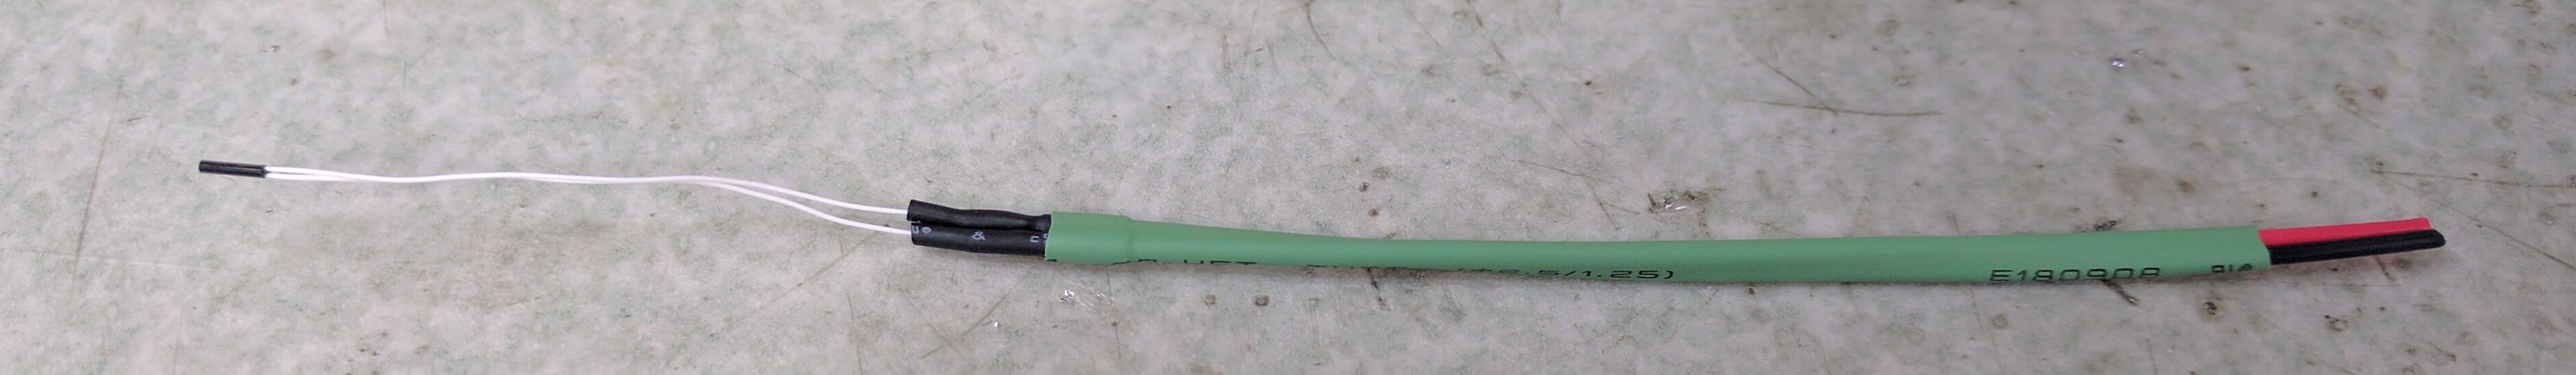
\includegraphics[width = \textwidth]{5.jpg}
	\caption[Thermistor Preparation.]{The thermistor sensor is prepared with additional wiring.}
	\label{fig:5}
\end{figure}ˆ 
\FloatBarrier

The thermistor sensor is then epoxied into the Thermal Region and encased in thermal paste to ensure accurate measurement. This step is pictured in Figure \ref{fig:6}.

\begin{figure}[!htb]
	\centering
	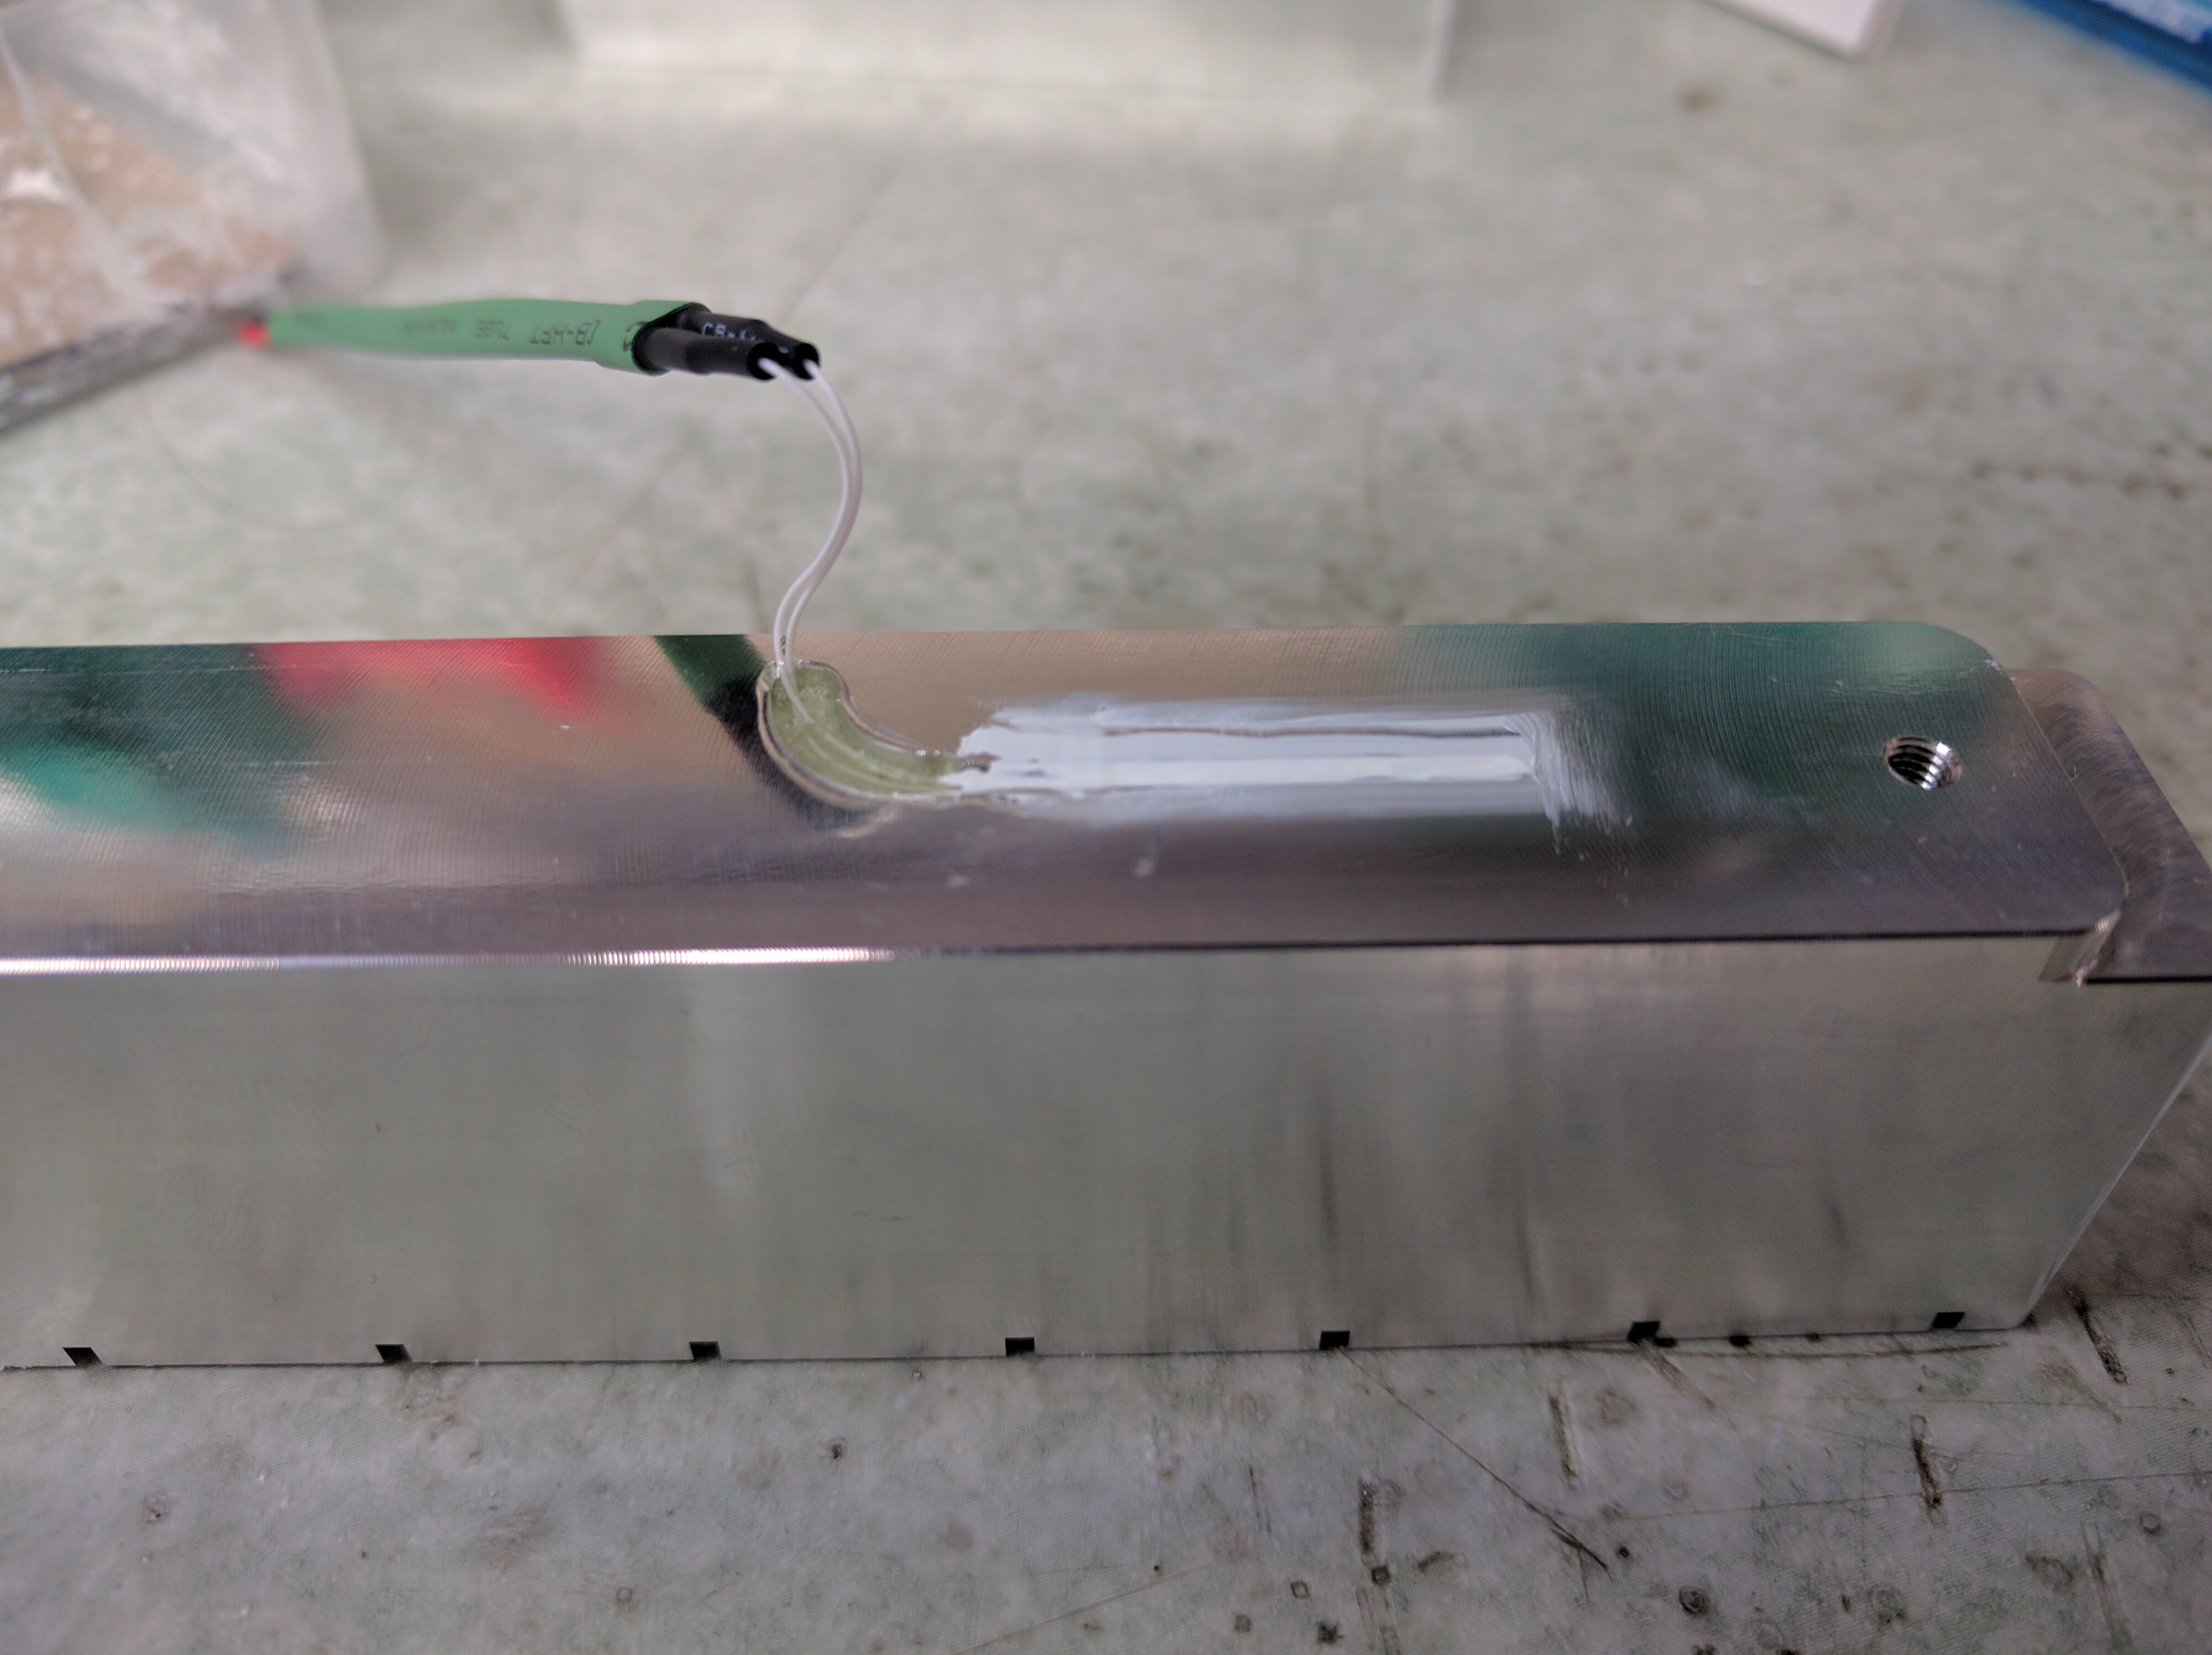
\includegraphics[width = \textwidth]{6.jpg}
	\caption[Thermistor Placement.]{The thermistor sensor placement in the Thermal Region.}
	\label{fig:6}
\end{figure}ˆ 
\FloatBarrier

The Thermal Region, Carrier and heat sink may now be fastened together via the two M3 bolts, with the torque specified in Section \ref{sec:mechdesign}. The MTX Cycler electronic board is also fixed to the device and the connections for the thermistor sensor, the TEC voltage and ground along with the communications connector for the Gene-Plex Extractor main board. This assembly is shown in Figure \ref{fig:7}. 

\begin{figure}[!htb]
	\centering
	\includegraphics[width = \textwidth]{7.jpg}
	\caption[Thermal Region and Board Assembly.]{The Thermal Region is then assembled onto the heat sink with the Carrier, along with the circuit board.}
	\label{fig:7}
\end{figure}ˆ 
\FloatBarrier

Finally, the circuit board cover may be fastened to the bottom of the module to complete the assembly. The completed Processor Module assembly is pictured in Figure \ref{fig:8}.

\begin{figure}[!htb]
	\centering
	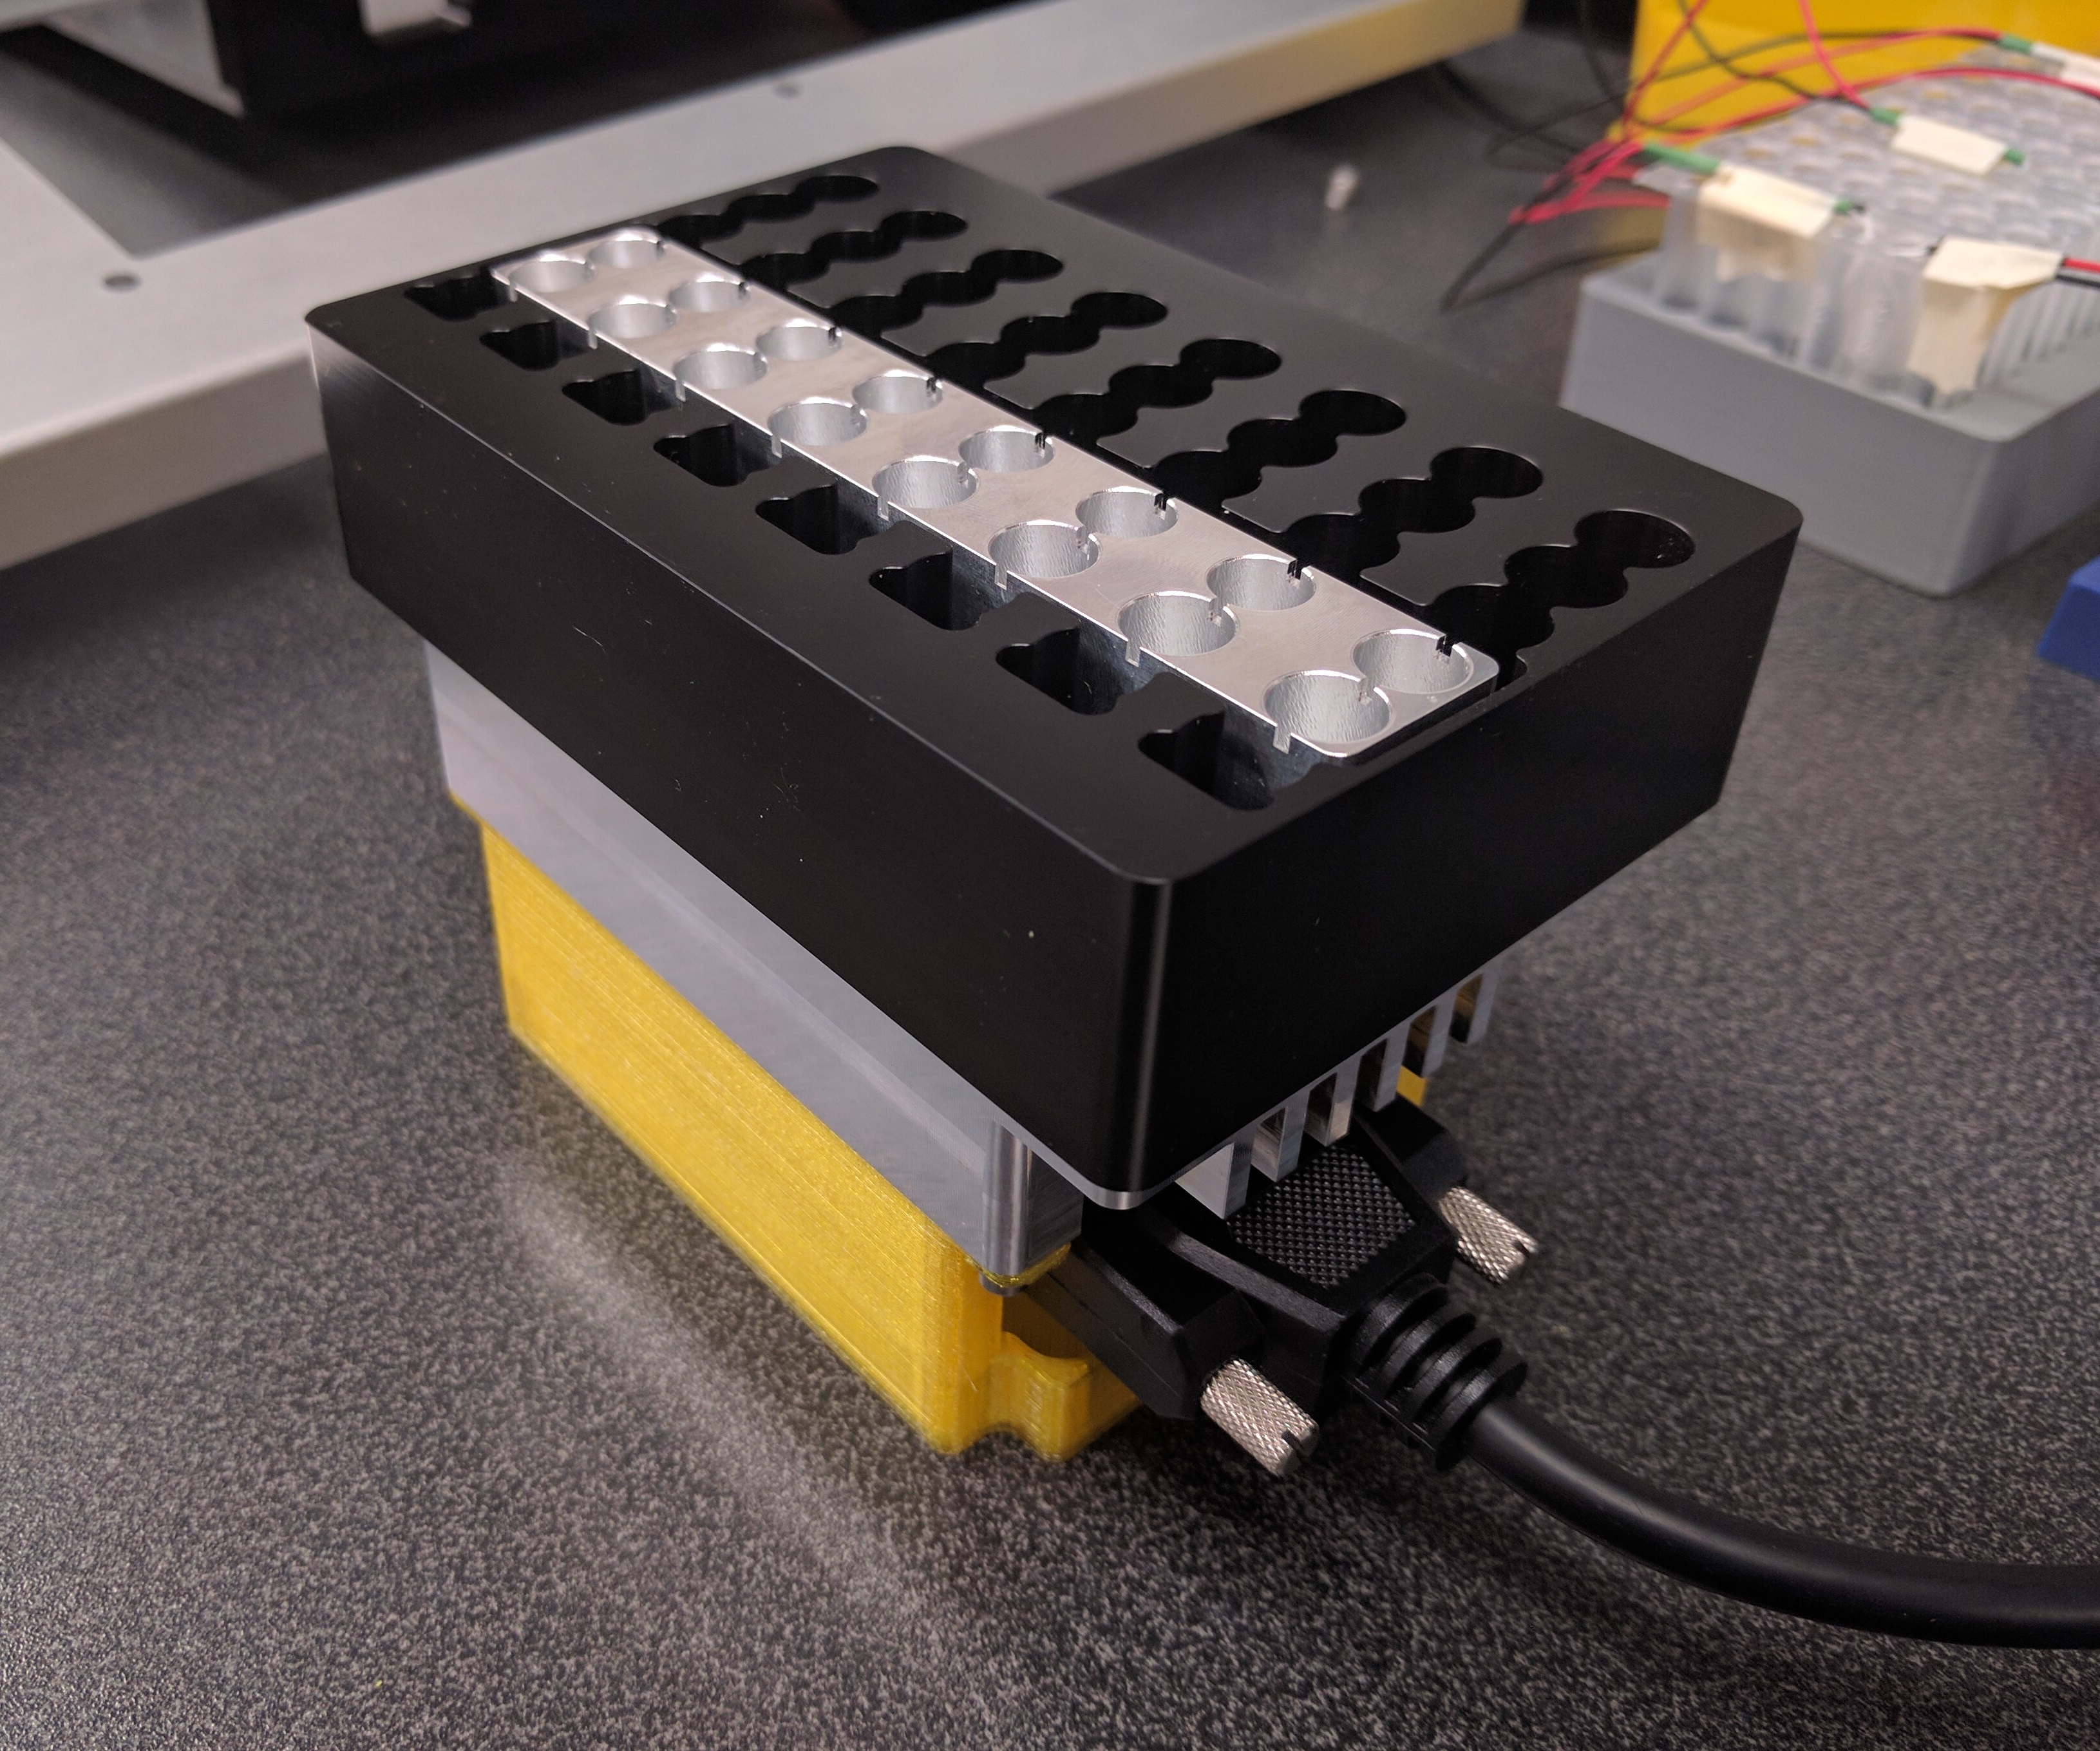
\includegraphics[width = \textwidth]{8.jpg}
	\caption[Assembled Processor Mpdule.]{The fully assembled Processor Module.}
	\label{fig:8}
\end{figure}ˆ 
\FloatBarrier

\subsection{Temperature Controller}
\label{sec:ControllerDesign}

\subsection{Magnetic Separation}

\section{Magnetic Separation Station}

\subsection{Magnetic Separation}

\subsection{Waste Disposal}